%%%%%%%%%%%%%%%%%%%%%%%%%%%%%%%%%%%%%%%%%
% Short Sectioned Assignment
% LaTeX Template
% Version 1.0 (5/5/12)
%
% This template has been downloaded from:
% http://www.LaTeXTemplates.com
%
% Original author:
% Frits Wenneker (http://www.howtotex.com)
%
% License:
% CC BY-NC-SA 3.0 (http://creativecommons.org/licenses/by-nc-sa/3.0/)
%
%%%%%%%%%%%%%%%%%%%%%%%%%%%%%%%%%%%%%%%%

%----------------------------------------------------------------------------------------
%	PACKAGES AND OTHER DOCUMENT CONFIGURATIONS
%----------------------------------------------------------------------------------------

\documentclass[paper=a4, fontsize=12pt, xcolor=dvipsnames]{scrartcl} % A4 paper and 11pt font size

% Biblatex

\usepackage[
style=nature,    % Zitierstil
isbn=false,                % ISBN nicht anzeigen, gleiches geht mit nahezu allen anderen Feldern
pagetracker=true,          % ebd. bei wiederholten Angaben (false=ausgeschaltet, page=Seite, spread=Doppelseite, true=automatisch)
maxbibnames=50,            % maximale Namen, die im Literaturverzeichnis angezeigt werden (ich wollte alle)
maxcitenames=3,            % maximale Namen, die im Text angezeigt werden, ab 4 wird u.a. nach den ersten Autor angezeigt
autocite=inline,           % regelt Aussehen für \autocite (inline=\parancite)
block=space,               % kleiner horizontaler Platz zwischen den Feldern
backref=false,              % Seiten anzeigen, auf denen die Referenz vorkommt
backrefstyle=three+,       % fasst Seiten zusammen, z.B. S. 2f, 6ff, 7-10
date=short,                % Datumsformat
backend = biber
]{biblatex}
\setlength{\bibitemsep}{1em}     % Abstand zwischen den Literaturangaben
\setlength{\bibhang}{2em}        % Einzug nach jeweils erster Zeile
\bibliography{report}  % Bibtex-Datei wird schon in der Preambel eingebunden

\usepackage[T1]{fontenc} % Use 8-bit encoding that has 256 glyphs
\usepackage{fourier} % Use the Adobe Utopia font for the document - comment this line to return to the LaTeX default

\usepackage{eufrak}
\usepackage{amsmath,amsfonts,amsthm} % Math packages
\usepackage{pgfplots}
\usepackage{wrapfig}
\usepackage{sidecap}
\usepackage{color, colortbl}  

\usepackage{afterpage}
%\usepackage[pass,showframe]{geometry} % just to show the margins
%\usepackage{booktabs}
%\usepackage{minted}

% Bibliographie auf deutsch
%\usepackage{harvard}
%\renewcommand{\harvardand}{und} 
\usepackage{caption}
\usepackage{xcolor}
\usepackage[utf8]{inputenc} 
%\usepackage[ngerman]{babel}

\usepackage{latexsym}
\usepackage{textcomp}
\usepackage[T1]{fontenc}
\usepackage{bm}% bold math
\usepackage{graphicx}
\usepackage{eso-pic}
\usepackage{caption}
\usepackage{subcaption}
\usepackage{verbatim}
\usepackage{epsfig}
\usepackage{framed,color}
\usepackage{placeins}   % FloatBarrier
\usepackage{float}   % places floats correctly
\usepackage[usenames,dvipsnames]{pstricks}
\usepackage{epsfig}
\usepackage{tikz}
\usepackage{sectsty} % Allows customizing section commands
\usepackage{hyperref}
\allsectionsfont{\normalfont\scshape} % Make all sections centered, the default font and small caps

\usepackage{fancyhdr} % Custom headers and footers
\pagestyle{fancy} % Makes all pages in the document conform to the custom headers and footers
\renewcommand{\headrulewidth}{0.0pt} % Remove header underlines
\renewcommand{\footrulewidth}{0pt} % Remove footer underlines

\setlength{\headheight}{13.6pt} % Customize the height of the header
\numberwithin{equation}{section} % Number equations within sections (i.e. 1.1, 1.2, 2.1, 2.2 instead of 1, 2, 3, 4)
\numberwithin{figure}{section} % Number figures within sections (i.e. 1.1, 1.2, 2.1, 2.2 instead of 1, 2, 3, 4)
\numberwithin{table}{section} % Number tables within sections (i.e. 1.1, 1.2, 2.1, 2.2 instead of 1, 2, 3, 4)

\setlength\parindent{0pt} % Removes all indentation from paragraphs - comment this line for an assignment with lots of text
\setcapindent{1cm} 
\setcounter{MaxMatrixCols}{50}
%----------------------------------------------------------------------------------------
%	TITLE SECTION
%----------------------------------------------------------------------------------------

\title{ 
\normalfont \normalsize 
\textsc{Albert-Ludwigs-University Freiburg} \\ [25pt] % Your university, school and/or department name(s)
\horrule{0.5pt} \\[0.4cm] % Thin top horizontal rule
\huge \textsc{Long half lifes} \\ % The assignment title
\horrule{2pt} \\[0.5cm] % Thick bottom horizontal rule
}


\author{Friedrich Schüßler and Volker Karle} % Your name

\date{\normalsize\today} % Today's date or a custom date
\DeclareGraphicsExtensions{.pdf,.png,.jpg}

%--------------------------------------------------------------------------------------------
% New Commands
%--------------------------------------------------------------------------------------------
\newcommand{\horrule}[1]{\rule{\linewidth}{#1}} % Create horizontal rule command with 1 argument of height

\interfootnotelinepenalty=10000

\begin{document}

\blendcolors*{!83}\color{black}
\maketitle
\begin{center}
 
\includegraphics[width=0.7\linewidth]{figures/unifreiburg}
\end{center}
\thispagestyle{empty}
\newpage
    {\pagestyle{plain}
    \thispagestyle{empty}
    \tableofcontents
    \thispagestyle{empty}
    \cleardoublepage}
\newpage


%----------------------------------------------------------------------------------------
%	PROBLEM 1
%----------------------------------------------------------------------------------------
% This file contains all the new commands defined 
% in order to facilitate the writing of the latex code. 
% It has to be loaded into the main .tex file at the beginning!

\newcommand{\nn}{\nonumber \\}
\newcommand{\beq}{\begin{equation}}
\newcommand{\eeq}{\end{equation}}
\newcommand{\beqn}{\begin{equation*}}   % equation without numbering
\newcommand{\eeqn}{\end{equation*}}
\newcommand{\bea}{\begin{eqnarray}}
\newcommand{\eea}{\end{eqnarray}}
\newcommand{\bean}{\begin{eqnarray*}}
\newcommand{\eean}{\end{eqnarray*}}
\newcommand{\bit}{\begin{itemize}}
\newcommand{\eit}{\end{itemize}}

\newcommand{\E}{\mathbf{E}}
\newcommand{\D}{\mathbf{D}}
\newcommand{\B}{\mathbf{B}}



\setcounter{page}{1}
\clearpage
\section{Introduction}
\label{sec:introduction}
\paragraph{Decay of Particles} is one of the most fundamental phenomenon
in physics and within this experiment we will have the chance
to get a hands-on introduction into the fascinating field of nuclear and radiochemistry. \\\\ 
The goal will be to find the half-lifes of two elements: \textbf{Samarium-147}, as an \textit{alpha ray}
source and \textbf{potassium-40} as \textit{beta ray} source. Firstly, in section~\ref{sec:theory}, 
we offer a short overview about the most important theoretical concepts we will be using.
In section~\ref{sec:setup} we will talk about the experimental setup and its 
functionality and after, in section~\ref{sec:measurements}, about our
own conduction of the measurements and their evaluation. Finally
we will give an appopriate interpretation of our results and conclude with
section~\ref{sec:conclusion}. For additional figures and the scanned records,
refer to the appendix, section~\ref{sec:appendix}.

\subsection{Theoretical Foundations}
When describing molecules in the framework of quantum mechanics, we are faced with the problem of 
finding solutions to the non-relativistic and time-independent Schrödinger-equation
\begin{equation}
    \hat{H} \psi = \Big[- \frac{\hbar^2}{2m} 
        \nabla^2 + \hat{V}(\mathbf{r}) \Big] \psi = E \psi
\end{equation}
where $\psi$ are eigenfunctions of the hamilton operator $\hat{H}$.
It is out of the scope of this introduction to give a complete
and comprehensive introduction into quantum mechanics, therefore
we will not only leave out the most important results, but
furthermore mention those kind of results without proof which
we need for further calculations. For the beginning it is
important to at least write down the characterisic properties
of the harmonic oscillator, in order to perturbate this
kind of potential onto a unharmonic oscillator, which will be
treated with secondorder perturbationtheory. After this we 
immedeatly come to the molecule orbitals, which we need
to resolve the energy levels being measured in this experiment.
\subsubsection{Harmonic Oscillator}
The potential for the harmonic oscillator is given as follwing:
\begin{equation}
    \hat{V}= \frac{m}{2} \omega^2 \hat{x}^2
\end{equation}
To solve this equation, the most convenient method is to
introduce different basis of operators in which it is very
convenient to write down the energy
~\cite{fliessbach2008quantenmechanik}, which we will not do here
but state the eigenvalues (with quantumnumber $\nu$)
of the energy without proof
(see also figure~\ref{fig:harmonic1}):
\begin{equation}
    H(\nu) = \left ( \nu + \frac{1}{2} \right )\hbar \omega 
    \quad \text{with $\nu\in \mathbb{N_0}$}
\end{equation}
where the wavefunctions
   are given by
   \begin{equation}
    \psi_n(x)= \left(\frac{m\omega}{\pi\hbar}
    \right)^\frac{1}{4}
\frac{1}{\sqrt{2^nn!}} H_n
\left(\sqrt{\frac{m\omega}{\hbar}} x \right)
e^{-\frac{1}{2}\frac{m\omega}{\hbar}x^2}
\end{equation}
and $H_n$ are the hermite polynomials: 
\begin{equation}
H_n(x)=(-1)^n e^{x^2}\frac{d^n}{dx^n}\left(e^{-x^2}\right) 
\end{equation}
\begin{figure}
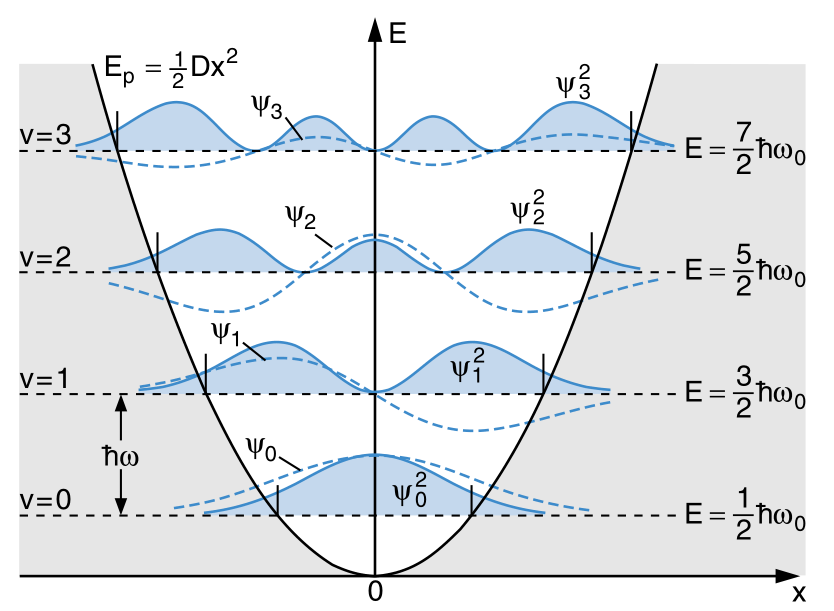
\includegraphics[width=15cm]{pics/harmonic1}
\caption{Energy levels of the harmonic oscillator with its 
    related wavefunctions\cite{Demtroeder1}.}
\label{fig:harmonic1}
\end{figure}
This potential is of outstanding importance for our experiment,
since the real potential will be aproximated in a region near
the minimum with a harmonic potential. 
To a few problems we can find the analytical solution
to the schrödingerequation, but to most
of the problems we need to approximate the solution with regards to an analyical
solution which is given. In the following sections we will introduce
the time-independent Perturbationtheory and give an example with the 
anharmonic oscillator how such an approximation can take place.
\subsubsection{Timeindependent Perturbationtheory}
We are following~\cite{fliessbach2008quantenmechanik}.
Lets assume we know the Eigenvalues and -functions of a specific
Hamiltonoperator $\hat{H_0}$ of the
unperturbed system (we further assume the eigenspaces to be
seperable, so we have no degeneracy. The case of degeneracy
can be done analogously) 
, numbered with $n\in \mathbb{N}$:

\begin{equation}
\hat{H_0} |n\rangle = \epsilon_n |n\rangle 
\end{equation}
and now we search for the solution of the perturbated Hamiltonian:
\begin{equation}
    \hat{H}|\psi \rangle = E|\psi \rangle 
\end{equation}
by means of the initial Hamiltonian:
\begin{equation}
    \hat{H} = \hat{H_0} + \lambda \hat{V}
\end{equation}
where we perturbate the original Hamiltonian with the Potential
$\hat{V}$ and give an approximate Soluation as long as Perturbation
is not of the same order of magnitude as $H_0$. 
The next step will be to apply this to the anharmonic 
Oscillator in order to get an estimation about the energyeigenvalues.
At first we have introduced a new parameter $\lambda$, which is the 
strength of the perturbation; for $\lambda = 1$ we have the problem
we want to solve, for $\lambda = 0 $ we arrive at the unperturbed
problem. Now we can expand in this parameter:
\begin{align}
    E_n(\lambda) &= \epsilon_n + \sum_{\nu =1}^{\infty} \lambda^\nu
    E_{n,\nu} \\ 
    |\psi_n(\lambda)\rangle &=
    |n\rangle + \sum_{\nu =1}^{\infty} \lambda^\nu
    |\psi_{n,\nu}(\lambda)\rangle
\end{align}
As result the solutions we are looking for will become:
\begin{align}
    E_n &= \epsilon_n + E_{n,1} + E_{n,2} + \cdots\\ 
    |\psi_n \rangle &= |n\rangle + |\psi_{n,1} \rangle + \cdots 
\end{align}
We assume for now that this series is converging and plug it into
the Schrödingerequation:
\begin{equation}
    (\hat{H_0} + \lambda \hat{V})
   \left( |n\rangle + \sum_{\nu =1}^{\infty} \lambda^\nu
        |\psi_{n,\nu}(\lambda)\rangle \right) =
\epsilon_n + \sum_{\nu =1}^{\infty} \lambda^\nu
    E_{n,\nu}  
    \left( |n\rangle + \sum_{\nu' =1}^{\infty} \lambda^{\nu'}
        |\psi_{n,\nu'}(\lambda)\rangle \right) 
\end{equation}
Now we can impose that the different powers of $\lambda$ have to
match on both sides and receive a set of equations:
\begin{align}
    \hat{H_0} |n\rangle &= \epsilon_n |n\rangle\\
    \hat{H_0} |\psi_{n,1}\rangle + \hat{V}|n\rangle &=
    \epsilon_n |\psi_{n,1}\rangle + E_{n,1}|n\rangle \label{eq:dev1}\\
    \hat{H_0} |\psi_{n,2}\rangle + \hat{V}|\psi_{n,1}\rangle &=
    \epsilon_n |\psi_{n,2}\rangle + E_{n,1}|\psi{n,1}\rangle 
    + E_{n,2}|n\rangle \label{eq:dev2}\
\end{align}
This set of equations yield recursive the Solutions of $E_{n,1}$,
$E_{n,2}$ and so on. Now we expand these single Wavefunctions 
into the new basis of energyeigenfunctions $|m \rangle$ with $m\in 
\mathbb{N}$:
\begin{equation}
    |\psi_{n,1}\rangle = \sum_{m=1}^{\infty} a_{nm} |m \rangle
    \label{eq:psi_expansion}
\end{equation}
We can plug this expansion now into into equation~\eqref{eq:dev1}:
\begin{equation}
    \sum_{m=1}^{\infty} (\epsilon_n - \epsilon_m) a_{nm} |m\rangle
    + E_{n,1} |n\rangle = \hat{V}|n \rangle
\end{equation}
With the Projection onto the dual eigenstate $\langle k|$ we can
use the orthonormality $\langle k | m \rangle = \delta_{m,k}$ 
of the energyeigenfunctions:
\begin{equation}
     (\epsilon_n - \epsilon_k) a_{nk} 
     + E_{n,1}\delta_{n,k}  = \langle k |\hat{V}|n \rangle
\end{equation}
For the case $k = n$ we get:
\begin{equation}
    E_{n,1} = \langle k |\hat{V}|n \rangle
\end{equation}
and for $k\neq m$:
\begin{equation}
    a_{n,k} = \frac{\langle k |\hat{V}|n \rangle}
    {\epsilon_n - \epsilon_k} \label{eq:a_nk}
\end{equation}
Equation~\eqref{eq:a_nk} together with~\eqref{eq:psi_expansion} 
gives us now:
\begin{equation}
    |\psi_{n}\rangle = |n\rangle + \lambda \sum_{m\neq n}^{\infty}
    \frac{\langle m |\hat{V}|n \rangle}{\epsilon_n - \epsilon_m}  
    |m \rangle + \lambda a_{n,n} + \mathcal{O}(\lambda^2)
\end{equation}
Now we can set $a_{n,n}=0$ (see footnote~\footnote{
Again we can use orthonormality:
\begin{equation*}
    1\overset{!}{=} \langle \psi_n|\psi_{n}\rangle 
    = \left | 1 + \lambda a_{nn} \right |^2 + \lambda^2
    \sum_{m\neq n}^{\infty}
    \left | \frac{\langle m |\hat{V}|n \rangle}
        {\epsilon_n - \epsilon_m} \right |^2 = 
    1 + \lambda (a_{n,n} + a^*_{n,n}) + \mathcal{O}(\lambda^2)
\end{equation*}
When $\lambda > 0 $ this results into:
\begin{equation*}
    a_{n,n} + a^*_{n,n} = 0 \Rightarrow \Re  [a_{n,n}] = 0
\end{equation*}
Since the Wavefunctions 
are invariant with respect to a phase $\phi$,
we can set without limitations $a_{nn}$ to zero.} for
further details) and we arrive
at:
\begin{equation}
    |\psi_{n}\rangle = |n\rangle + \lambda \sum_{m\neq n}^{\infty}
    \frac{\langle m |\hat{V}|n \rangle}{\epsilon_n - \epsilon_m}  
    |m \rangle  + \mathcal{O}(\lambda^2)
\end{equation}
For the Energy we can make use of the third equation and go to
the second order:
\begin{equation}
|\psi_{n,2}\rangle  = \sum_{m=1}^{X} b_{n,m} |m \rangle 
\end{equation}
We can plug this analogously into equation~\eqref{eq:dev2} and
arrive at:
\begin{equation}
 \sum_{m}^{\infty} (\epsilon_n - \epsilon_m) b_{nm} |m\rangle +
 \sum_{m}^{\infty} E_{n,1} a_{n,m} |m \rangle + E_{n,2} |n \rangle =
 \sum_{m}^{\infty} a_{n,m} \hat{V} |m \rangle
\end{equation}
Where again we use the orthonormality. For $k=n$ we get:
\begin{equation}
    E_{n,2} = \sum_{m}^{\infty} a_{n,m} \langle n |\hat{V}|m\rangle
= \sum_{m\neq n}^{\infty}\frac{|\langle n | \hat{V} | m \rangle |^2}
    {\epsilon_n - \epsilon_m}
\end{equation}
For $k\neq n$ we would arrive at the explicit formula for $b_{n,m}$
but this is not necessary for the further computations.
As final result we therefore get:
\begin{align}
    E_n &\approx \epsilon_n + \langle n|\hat{V} | n \rangle +
\sum_{m\neq n}^{\infty}\frac{|\langle n | \hat{V} | m \rangle |^2}
    {\epsilon_n - \epsilon_m} \\
    |\psi_n \rangle &\approx 
    |n\rangle + \sum_{m\neq n}^{\infty}
    \frac{\langle m |\hat{V}|n \rangle}{\epsilon_n - \epsilon_m}  
    |m \rangle 
\end{align}
\subsection{The anharmonic oscillator}
Lets assume we have solved the harmonic oscillator with 
\begin{align}
    \hat{H_0} &= \frac{\hat{p}^2}{2m} 
    + \frac{1}{2} m \omega_0^2\hat{x}^2 \\
    \hat{H_0}|n \rangle &= \epsilon_n |n \rangle \\
    \epsilon_n &= \hbar \omega_0 \left (n+ \frac{1}{2} \right)
\end{align}
Now perturbe this system with a kubic potential potential:
\begin{equation}
\hat{V} =\lambda \hat{x}^3
\end{equation}
Hence we can use the perturbation theory in linear order.
Since the parity of $\hat{V}$ is odd, the expectation value has 
to be zero:
\begin{equation}
    E_{n,1} = \lambda \langle n | \hat{x}^3 | n \rangle = 0 
\end{equation}
The wavefunctions have to be corrected as follows:
\begin{equation}
    |\psi_{n,1} \rangle = \sum_{m\neq n}^{\infty}
    \frac{\langle m |\hat{V}|n \rangle}{\epsilon_n - \epsilon_m}  
    |m \rangle 
    = \frac{\lambda}{\hbar \omega}
    |\psi_{n,1} \rangle = \sum_{m\neq n}^{\infty}
    \frac{\langle m |\hat{x}^3|n \rangle}{\epsilon_n - \epsilon_m}  
    |m \rangle 
\end{equation}
Now we have to calculate the matrix elements. Therefore we
introduce the creation- and annihilationoperator 
which are defined by $\hat{x}$:
\begin{equation}
    \hat{x} = \sqrt{\frac{\hbar}{2m\omega}}(\hat{a}^\dagger +
        \hat{a})
\end{equation} 
Now we can calculate iteratively the matrixelements
\footnote{
    Here we make use how $\hat{a}$ and $\hat{a}^\dagger$ act 
    on the eigenfunctions $|n\rangle$:
\begin{align*}
    \hat{x}|n'\rangle = \sqrt{\frac{\hbar}{2m\omega}}
    \left ( \sqrt{n' + 1}|n'+1\rangle 
        + \sqrt{n'}|n' - 1 \rangle \right ) 
\end{align*}
Applying once more:
\begin{align*}
\hat{x}^2|n'\rangle = \frac{\hbar}{2m\omega}
\left ( \sqrt{(n' + 1)(n' + 2)}|n'+2\rangle 
            + (2n' + 1) |n' \rangle
            + \sqrt{(n'(n'-1)}|n' - 2 \rangle \right ) 
\end{align*}
And applying for the third time:
\begin{align*}
    \hat{x}^3|n'\rangle &= \sqrt[3]{\left (\frac{\hbar}{2m\omega}\right )^2}
( \sqrt{(n' + 1)(n' + 2)(n'+3)}|n'+3\rangle 
    + 3 \sqrt{(n'+1)^3}|n' +1 \rangle  \\
 &+ 3 \sqrt{(n')^3}|n' -1 \rangle   
            + \sqrt{(n'(n'-1)(n'-2)}|n' - 3 \rangle  ) 
\end{align*}
Now this yields the matrixelements which we need:
\begin{align}
    \langle n | \hat{x}^3 | n' \rangle &=  
    \sqrt{\left (\frac{\hbar}{2m\omega}\right)^3}
( \sqrt{(n' + 1)(n' + 2)(n'+3)}\delta_{n,n'+3} 
    + 3 \sqrt{(n'+1)^3}\delta_{n,n'-1}  \\
    &+ 3 \sqrt{(n')^3}\delta_{n,n'-1}   
    + \sqrt{(n'(n'-1)(n'-2)}\delta_{n,n'-3}  ) 
\end{align}

}. After applying the justified indices, since only $n'=n\pm 1$ and
$m = n \pm 3 $ are not zero, we arrive at:
\begin{equation}
\begin{aligned}
    |\psi_{n,1} \rangle &= \frac{\lambda}{\hbar \omega}
    \sqrt{\left(\frac{\hbar}{2m\omega}\right)^3}
    ( -\frac{1}{3}\sqrt{(n + 1)(n + 2)(n+3)}|n+3\rangle 
    - 3 \sqrt{(n+1)^3}|n +1 \rangle  \\
 &+ 3 \sqrt{(n)^3}|n -1 \rangle  
    +\frac{1}{3} \sqrt{(n(n-1)(n-2)}|n - 3 \rangle  ) 
\end{aligned}
\end{equation}
We can also calculate the energy corrections:
\begin{equation}
    E_{n,2} = \langle n | \hat{V} | \psi_{n,1} \rangle 
    = \lambda \langle n | \hat{x}^3 | \psi_{n,1} \rangle 
\end{equation}
Which yields:
\begin{equation}
\begin{aligned}
    E_{n,2} &= \frac{\hbar^2 \lambda^2}{2 m^3 \omega ^4}
    \left[-\frac{1}{3}(n+1)(n+2)(n+3)
        -9(n+1)^3 + 9n^3 + \frac{1}{3}n(n-1)(n-2)
        \right ] \\
    &= -\frac{\hbar^2 \lambda^2}{2 m^3 \omega ^4}
    \left[ 30n^2+ 30n + 11 \right ]\\
    &= -\frac{30 \hbar^2 \lambda^2}{2 m^3 \omega ^4}
    \left[\left(n + \frac{1}{2} \right)^2 + \frac{11}{30} \right ]\\
\end{aligned}
\end{equation}
If we had a look at the closed form for all orders, we would
notice the possibility to expand the Energy Difference in terms
of powers of the original Energy $(n+\frac{1}{2})$ which we will
state here without proof:
\begin{equation}
    E_n = \hbar \omega_{0,0} \left(n + \frac{1}{2} \right) 
    - \hbar \omega_{0,1} \left(n + \frac{1}{2} \right)^2  
    + \hbar \omega_{0,2} \left(n + \frac{1}{2} \right)^3  
    + \cdots
\end{equation}
We did not include the small derivation independent of $n$,
since we will look only at energydifferences. Notice that
the final result is only valid for a small, odd Perturbation. 
\subsubsection{Energylevels and Wavefunctions
    of two-atomic molecules}

First we will write down the full Equations of the two-atomic
molecule and investigate after which parts we can further
simplify (This whole derivation will follow \cite{staatsexamen}):
\begin{equation}
        \hat{H}\psi = E\psi 
\end{equation}
Where we can expand the Hamiltonian in the position-space,
where we already split into the electrons ($i$) and the 
two nucleons $A$ and $B$:
\begin{equation}
    \hat{H} = \frac{-\hbar^2}{2} 
        \underbrace{\left(
        \sum_{i}{\frac{\nabla_i^2}{m_e}}
        +\frac{\nabla_A^2}{M_A} +\frac{\nabla_B^2}{M_B}
\right)}_{
\substack{\text{kinetic energy}\\\text{of electrons and nucleons}}}
+ \underbrace{\sum_{i>j}{\frac{e^2}{|r_i - r_j|}}
    }_{\substack{\text{potential energy}\\\text{electron-electron}}}
 - \underbrace{\sum_{i}{\frac{Z_A e^2}{|r_i - r_A|}}
 }_{\substack{\text{potential energy}\\\text{electron-nucleon $A$}}}
 - \underbrace{\sum_{i}{\frac{Z_B e^2}{|r_i - r_B|}}
 }_{\substack{\text{potential energy}\\\text{electron-nucleon $B$}}}
 +  \underbrace{\frac{Z_A Z_B e^2}{|r_A - r_B|}
 }_{\substack{\text{potential energy}\\\text{nucleon $A$ - nucleon $B$}}}
\end{equation}
Now we split the electronsolutions and the nucleonsolutions such
that the solutions of the electrons change only little when the
distance of the nucleons change, which is known as the
\textsc{BORN-OPPENHEIMER}-Approximation \cite{staatsexamen}:
\begin{align}
    \psi &= \psi_E ( \cdots r_i \cdots) \psi_N(r_A, r_B) \\
    \hat{ H}_E\psi_E &= \left(- \sum_{i}{\frac{\hbar^2\nabla_i^2}{2m_e}}
    + \sum_{i>j}{\frac{e^2}{|r_i - r_j|}}
    - \sum_{i}\frac{Z_A e^2}{|r_i - r_A|}
    - \sum_{i}\frac{Z_B e^2}{|r_i - r_B|}
    + 
    \right ) \psi_E = 
 E_E \psi_E \\
 \hat{H}_N\psi_N &= \left (
 -\frac{\hbar^2\nabla_A^2}{2M_A} -\frac{\hbar^2\nabla_B^2}{2M_B}
    - \sum_{i}\frac{Z_A e^2}{|r_i - r_A|}
    - \sum_{i}\frac{Z_B e^2}{|r_i - r_B|}
 + \frac{Z_A Z_B e^2}{|r_A - r_B|}
 \right ) \psi_N
=  E_N \psi_N 
\end{align}
Where we fixed the positions for the Hamiltonian
of the electrons such that they are not included in the
wavefunction. The interaction between electrons and the nucleons
will not be neglected since the Wavefunctions $\psi_E$ are still
dependend of the distance between the nucleons $r$. 
\par
The obvious problem arises when trying to solve these equations,
since it is not possible without great difficulties. 
The next step is to build up trialsolutions of $\psi_E$, 
consisting of solutions when there is only one electron and a
nucleon. These solutions are called one-electron orbital wave
and will be abbreviated
with \textit{MO} (\textit{Molecule orbital}) and the trialsolutions
will be built up upon linear combinations of those
(\textit{Linear combinations of atomic orbitals} method,
\textit{LCAO}). This method was first introduced 1929 by 
Sir John Lennard-Jones and has to be used with caution, since
it is only in certain limits applicable. The parameters which
appear in these combinations can be constrained by 
expectationvalues measured in experiments.
Now we will turn our attention to the movement of nucleons.
Since in our case we only have two of them, we can perform 
a coordinatetransform to the normal coordinates with a fictional
nucleon with mass
\begin{equation}
    \mu = \frac{M_A M_B}{M_A + M_B}
\end{equation}
so that our new Schrödingerequation with the wavefunction of the
fictional nucleon will look like:
\begin{equation}
    \nabla^2 \psi_N + \frac{2\mu}{\hbar^2} 
    \left[ E - V(r) \right] = 0 
\end{equation}
The Laplaceoperator written in spherical coordinates will yield
the spherical harmonics as eigenfunctions, so we can use a 
seperational ansatz for our wavefunction:
\begin{equation}
    \psi_N(r,\theta,\rho) = \frac{1}{r} S(r)Y(\theta,\rho)
\end{equation}
with the corresponding
differentialoperator, where $J\in \mathbb{N}_0$
corresponds to the Quantumnumber of the total angular momentum:
\begin{equation}
    \frac{\partial}{\sin\theta \partial \theta}\left (\sin\theta
    \frac{\partial Y}{\partial \theta}\right ) +
\frac{1}{\sin^2\theta} \frac{\partial^2 Y}{ \partial\rho^2}
 + J(J+1)Y = 0
\end{equation}
Thus we can split the rest of the wavefunction into the 
radial component of the Operator:

\begin{equation}
    \frac{d^2 S}{dr^2} + \frac{2\mu}{\hbar^2}
\left ( E - V(r) - \frac{J(J+1)\hbar^2}{2\mu r^2} \right ) S =0 
\end{equation}

If there is no further degeneracy (for instance due to not
considered interactions like spin) we can in theory write
down the Energyeigenvalues in terms of the two Quantumnumbers
$nu$ and $J$:
\begin{equation}
    E = E_{\nu,J}
\end{equation}
Practically this is not possible, so we look at two extrem cases.
\paragraph{The rigid Rotator} is based on the approximation to
fix the range of the two nuclei ($r =$const.) and so we only
look at $V(r)=0$ and $\frac{S(r)}{r} = 1$. We immedeatly get
the solution (since the sphericalharmonics already resolved
the eigenvalues):
\begin{equation}
    E = \frac{J(J+1)\hbar^2}{2\mu r^2}
\end{equation}
\paragraph{The rotationless Oscillator} just neglects the terms
arising from rotation, which is, looking at the lengthscale of
the former calculated eigenvalues, not inopportune.
The Operator then becomes:
\begin{equation}
    \frac{d^2 S}{dr^2} + \frac{2\mu}{\hbar^2}
    \left ( E - V(r) ) = 0 \right )
\end{equation}
The Eigenfunctions and -values are now very dependent on the 
potential energy $V(r)$ which is until now not a known 
potential, because it includes the repulsion due to the
pauliprinciple of the electronorbits as well as the attraction
of the charges. Furthermore the physical nature of dissociation
of the two nucleons also has to be encoded into it.
It is not possible to solve the potential analytically, but 
we will start to write down the properties already known:
\begin{itemize}
        \item Pauliprinciple:
            $\lim\limits_{r \rightarrow 0}{V(r)} = \infty $
        \item Dissociated nucleons:
$\lim\limits_{r \rightarrow \infty}{V(r)} = const. $
\item Before the Dissociation: Attraction of the nucleons with
    the maximal attraction at $r_e$ and the Dissociationenergy
    $D_e$ defined by 
    $ \lim\limits_{r \rightarrow \infty}{V(r)} - V(r_e)=: D_e$ 
\end{itemize}
The idea is now to capture this properties into the coefficients
of the taylored Potential and by doing so resolving the principle
physical behavior:
\begin{equation}
    V(r) = V(r_e) 
   + \frac{\partial V(r)}{\partial r}|_{r=r_e}(r - r_e)
   + \frac{\partial^2 V(r)}{2!\partial r^2}|_{r=r_e}(r - r_e)^2
   + \frac{\partial^3 V(r)}{3!\partial r^3}|_{r=r_e}(r - r_e)^3
   + \cdots
\end{equation}
As first approximation for energies near the minimum $r=r_e$ we
can finally use the harmonic potential. The constant term
$V(r_e)$ can be dropped since we are only interested in 
potential differences.
\begin{equation}
    V_{harm}(r) =
    \frac{\partial^2 V(r)}{2\partial r^2}|_{r=r_e}(r - r_e)^2
    =: \frac{k_e}{2}(r-r_e)^2
\end{equation}
Following this approach we can use the energyeigenvalues of the
harmonic oscillator in order to approximate
the vibrational states $\nu$:
\begin{equation}
    E_\nu =\sqrt{\frac{k_e}{\mu}}\hbar \left (\nu
        + \frac{1}{2}\right )
\end{equation}
In order to chose a more convenient unit we transform this
equation into $cm^{-1}$:
\begin{equation}
    G_{harm}(\nu) = \frac{E}{hc} = \omega_0 (\nu + \frac{1}{2})
    \quad \text{with the frequency} \quad
    \omega_0 = \frac{1}{2\pi c} \sqrt{\frac{k_e}{\mu}}
\end{equation}
The wider we leave the regime around $r_e$, speaking about 
higher vibrational states, the worse approximation with a harmonic
oscillator becomes. Qualitatively this is the case when energies
come nearer to the dissociation energy. An adhoc solution is 
to treat this with the already mentioned perturbationtheory in such
a way that we use the condition
\begin{equation}
    \frac{\partial V(r)}{\partial r}|_{r=r_e}        \gg
    \frac{\partial^2 V(r)}{2!\partial r^2}|_{r=r_e}  \gg
    \frac{\partial^3 V(r)}{3!\partial r^3}|_{r=r_e}  
    \cdots
\end{equation}
and can therefore justify the Ansatz:
\begin{equation}
    G(\nu) = \omega_e (\nu + \frac{1}{2} ) 
    - \omega_e x_e (\nu + \frac{1}{2} ) ^2 
    + \omega_e y_e (\nu + \frac{1}{2} ) ^3 
    - \omega_e z_e (\nu + \frac{1}{2} ) ^4 
    + \cdots 
\end{equation}
Since in the experiment it is clearly impossible to seperate
the incoming higher frequencies, we will treat $\omega_e x_e$ as 
one variable, similarily to the others, where they also connected
on lengthscales by
\begin{equation}
    \omega_e \gg \omega_ex_e \gg \omega_e y_e \cdots 
\end{equation}
As before we can shift the equations to make them more convenient,
in this case to scale them to the zeroenergy
\begin{equation}
    G \mapsto G_0 := \left [G-G(0) \right ] 
        \quad \text{which is given by}
    \quad G(0)=\frac{1}{2}\omega_e - \frac{1}{4}\omega_e x_e 
    + \frac{1}{8} \omega_e y_e + \cdots 
\end{equation}
So we get for the shifted term:
\begin{equation}
    G_0(\nu) = 
\end{equation}
\clearpage



\section{Setup and procedure}
First we give an overview of the program which constitutes the experiment. In another subsection, 
we give a describtion of the setup used. 
\subsection{Procedure}
The procedure of measurements consists of the following six points:
\begin{enumerate}
    \item 
        \textbf{Assessing the detectors and probe at hand with the oscilloscope:}
        We measure the signals of the preamplifier (PA) as wel as uni- and bipolar outputs of 
        main amplifier (MA) at the oscilloscope. With this signal, we calculate the ascending time 
        of the signal.
    \item 
        \label{it:task2}
        \textbf{recording the energy spectrum of $^{57}$Co and $^{241}$Am:}
        The multichannel analyzer (MA) we measure the energy spectrum of both probes 
        for ca. 10 minutes. With the $^{57}$Co sample, we test the sensibility of each detector
        and the optimal positioning of the sample (which is not symmetric). After assigning the 
        channel-energy relationship based on the knowledge of some peaks, we interprete the other visible peaks.
    \item
        \textbf{setting the energy windows:}
        In this step, we restrict the events passed by the single channel analyzer (SCA) to those 
        of the 14.4 keV and 122 keV photons, respectively.
    \item
        \textbf{measuring the delayed coincidences:}
        Using the Time-to-Amplitude converter (TAC), we record the delays between 14.4 keV and 122 keV 
        events. Since the 14.4 keV photon is only emitted in 10 \% of the cases, we use this signal to start the 
        TAC, and stop with the delayed 122 keV photon, expecting to drastically reduce the dead time of the 
        measurement.
    \item
        \textbf{measuring the background (random coincidences):}
        Taking out the delay of the 122 keV signal and further introducing a delay on the 14.4 keV signal, 
        we measure the background. 
    \item
        \textbf{time calibration of Time to Amplitude converter (TAC):}
        In order to correlate measured channel and the respective time delay, we measure the channel 
        assigned by TAC and MCA corresponding to a known delay and perform a fit a linear function between 
        the two quantities. This correspondance will be used in the anaylsis of the delayed coincidences. 
\end{enumerate}


\subsection{Experimental setup}
The setup of the experiment consists of a fixed part with probe and a detector at each side 
as well as a part with the electronics. The devices are adapted to each part, as described below. 

A photo of the two detectors and the probe is shown in figure \ref{fig:position_1}. The given setup also 
defines position 1, later referred to as "Pos1" (see table \ref{tab:config2}). Position 2 ("Pos2") corresponds 
to the probe rotated by $180^\circ$. From its geometry, one can already suspect that the number of photons 
that can be measured from either direction is not equal. A similar condition is true for the detectors:
Already on the first glance, it is clear that the two are not of the same model. In fact, the left detector 
is an older model and suspected to be less sensitive. A more quantitative statement will be made in the 
of the second part of the experiment (see \ref{it:task2}).

\begin{figure}[H]
    \centering
    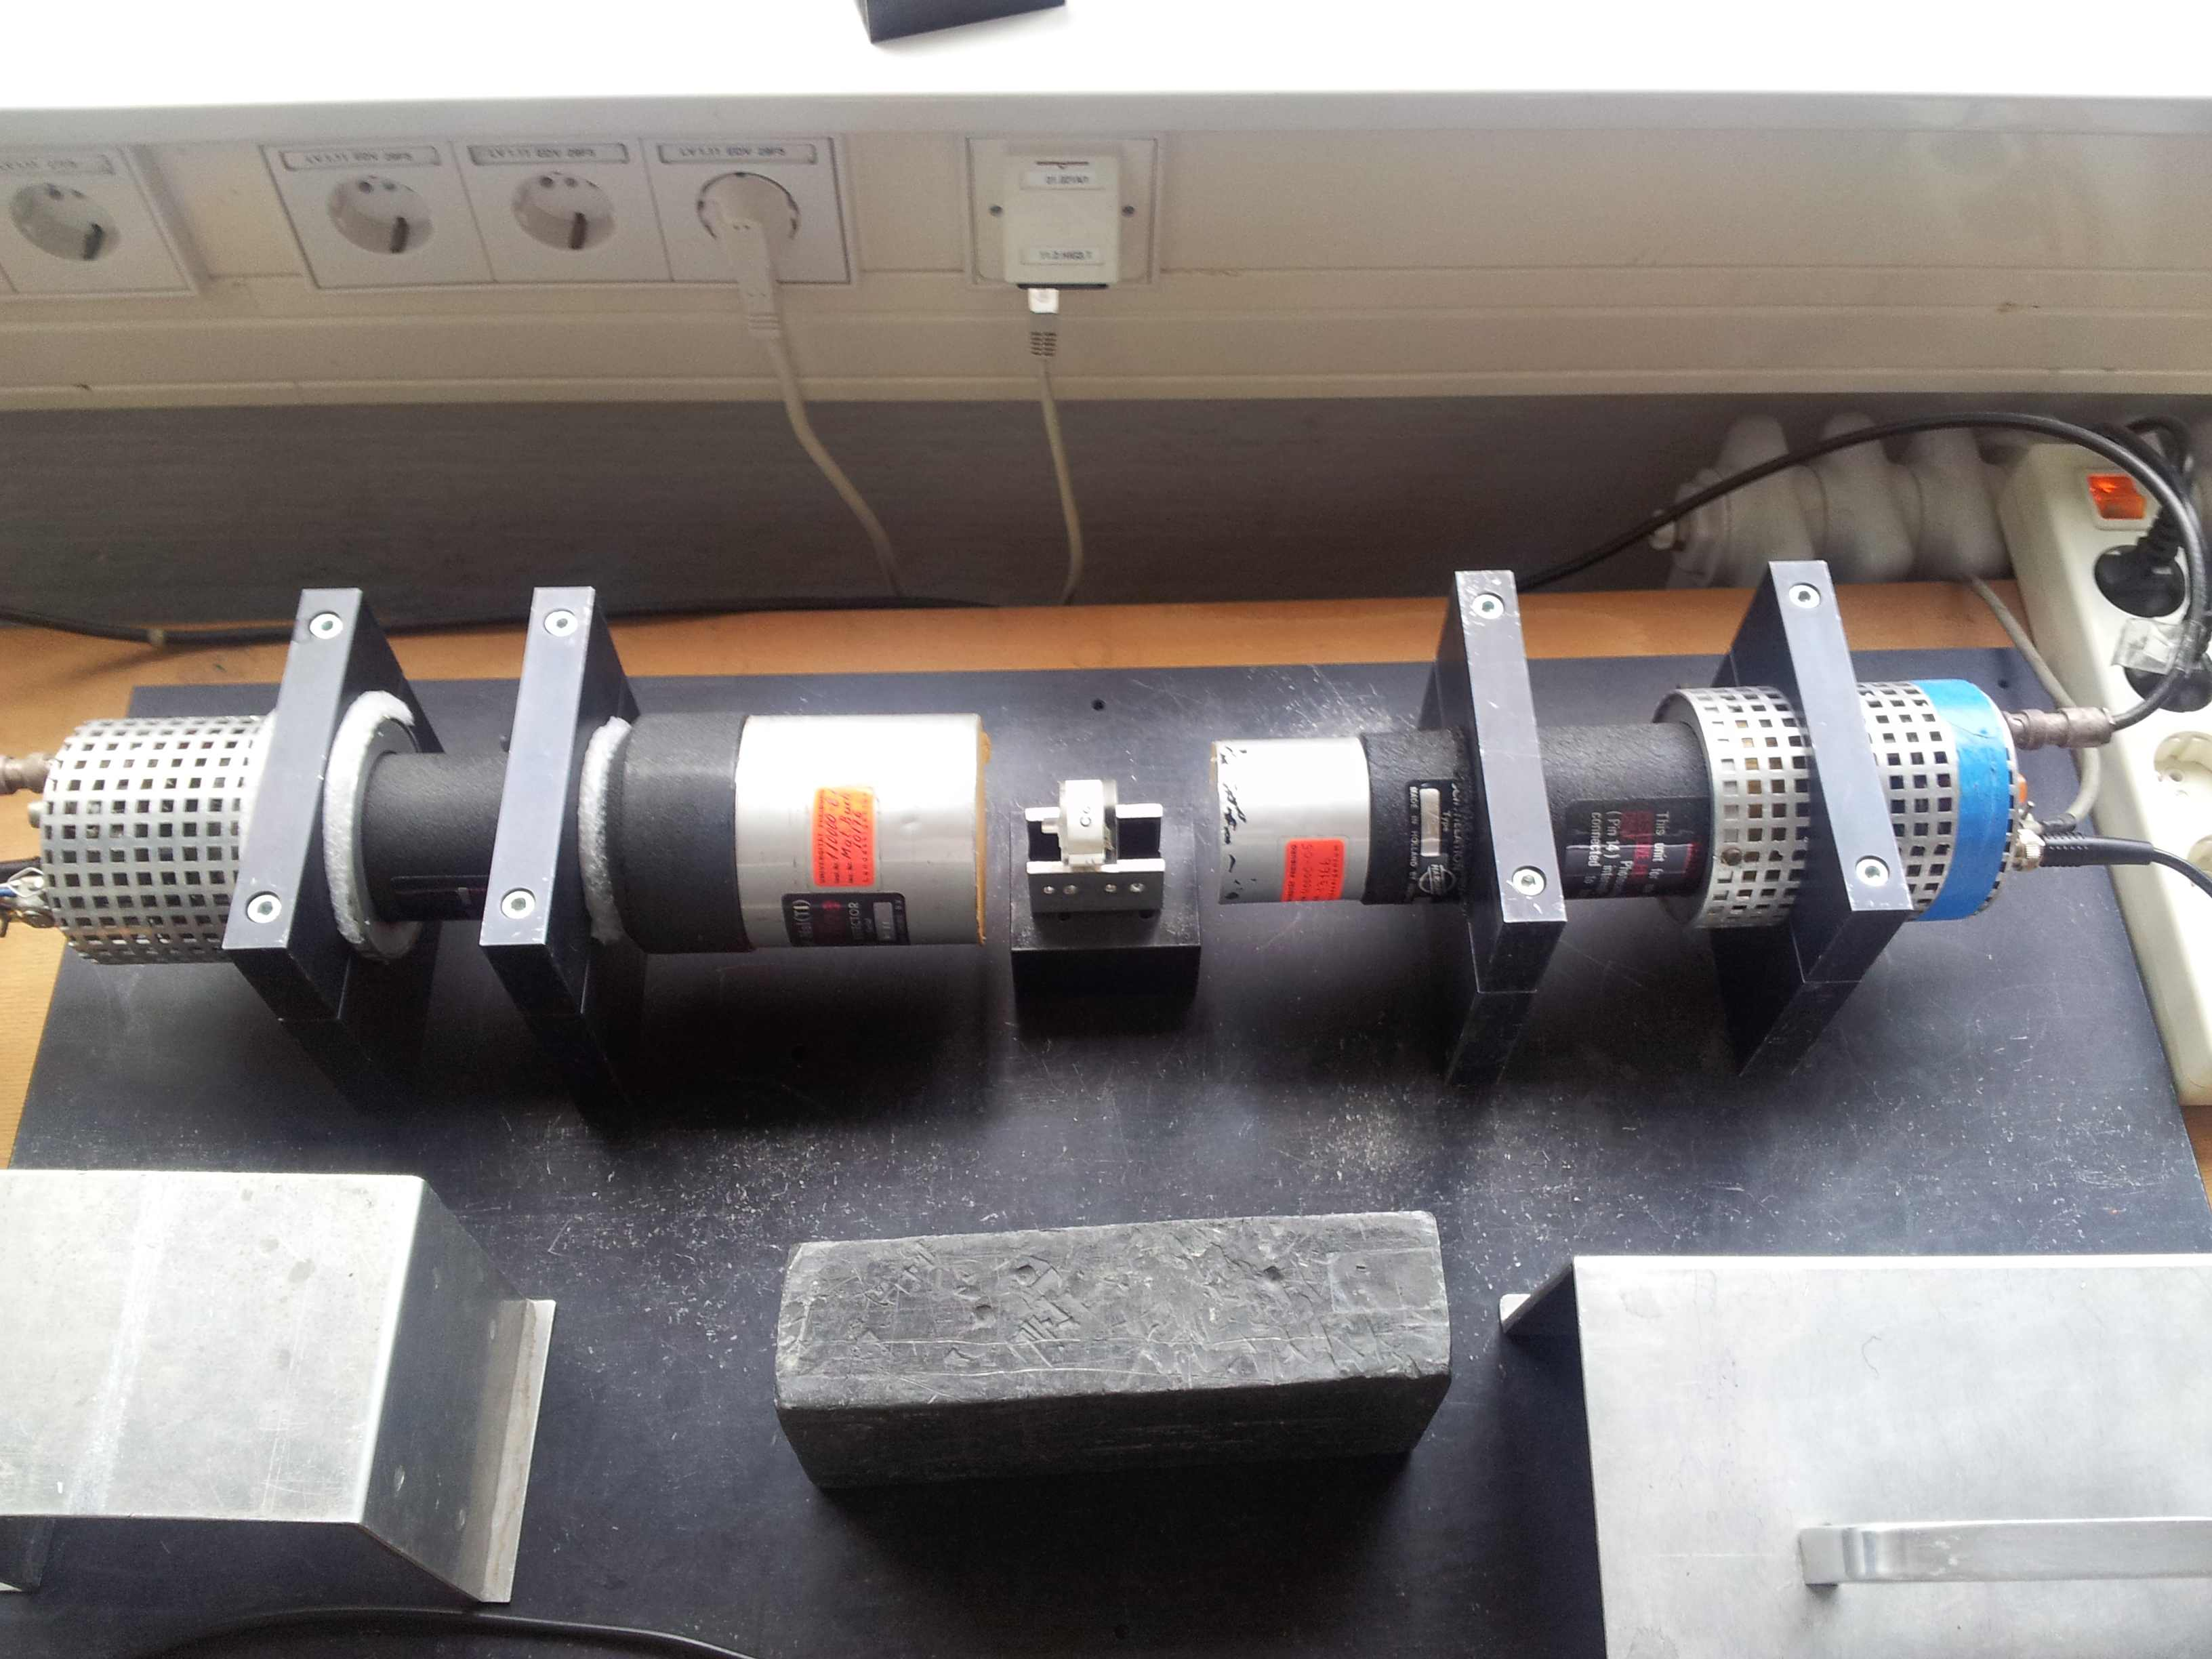
\includegraphics[width=0.8\linewidth]{figures/position_1.jpg}
    \caption{
        Photo of the $57$^Co probe and the two detectors with the setup used in the 
        experiment. The orientation of the probe is the one used for the measurement of 
        the delayed coincidences, with the larger opening facing the right detector. 
        During the measurements, the probe is isolated by the 
        }
    \label{fig:position_1}
\end{figure}




\section{Measurements}
\label{sec:measurements}

\subsection{Preparations and calibration of the setup}
\label{sub:preparations_and_calibration_of_the_setup}
\subsubsection{Controlling the setup with the oscilloscope}
\label{ssub:Controlling the setup with the oscilloscope}
See Table~\ref{tab:config} for the first configuration. 
First we measured the signal from the detector and Photomultiplier. We noticed
that the peaks of shape were at irregular points in time. We exchanged the left for the right side
of the photomultiplier, but did not observe a crucial dependence. Also rotating the sample did not
change the result significantly. Now we removed the oscilloscope and appended the Multichannelanalyzer,
in order to measure the energy spectrum. \\
\\
 \begin{minipage}{\textwidth}
  \begin{minipage}[b]{0.49\textwidth}
    \centering
    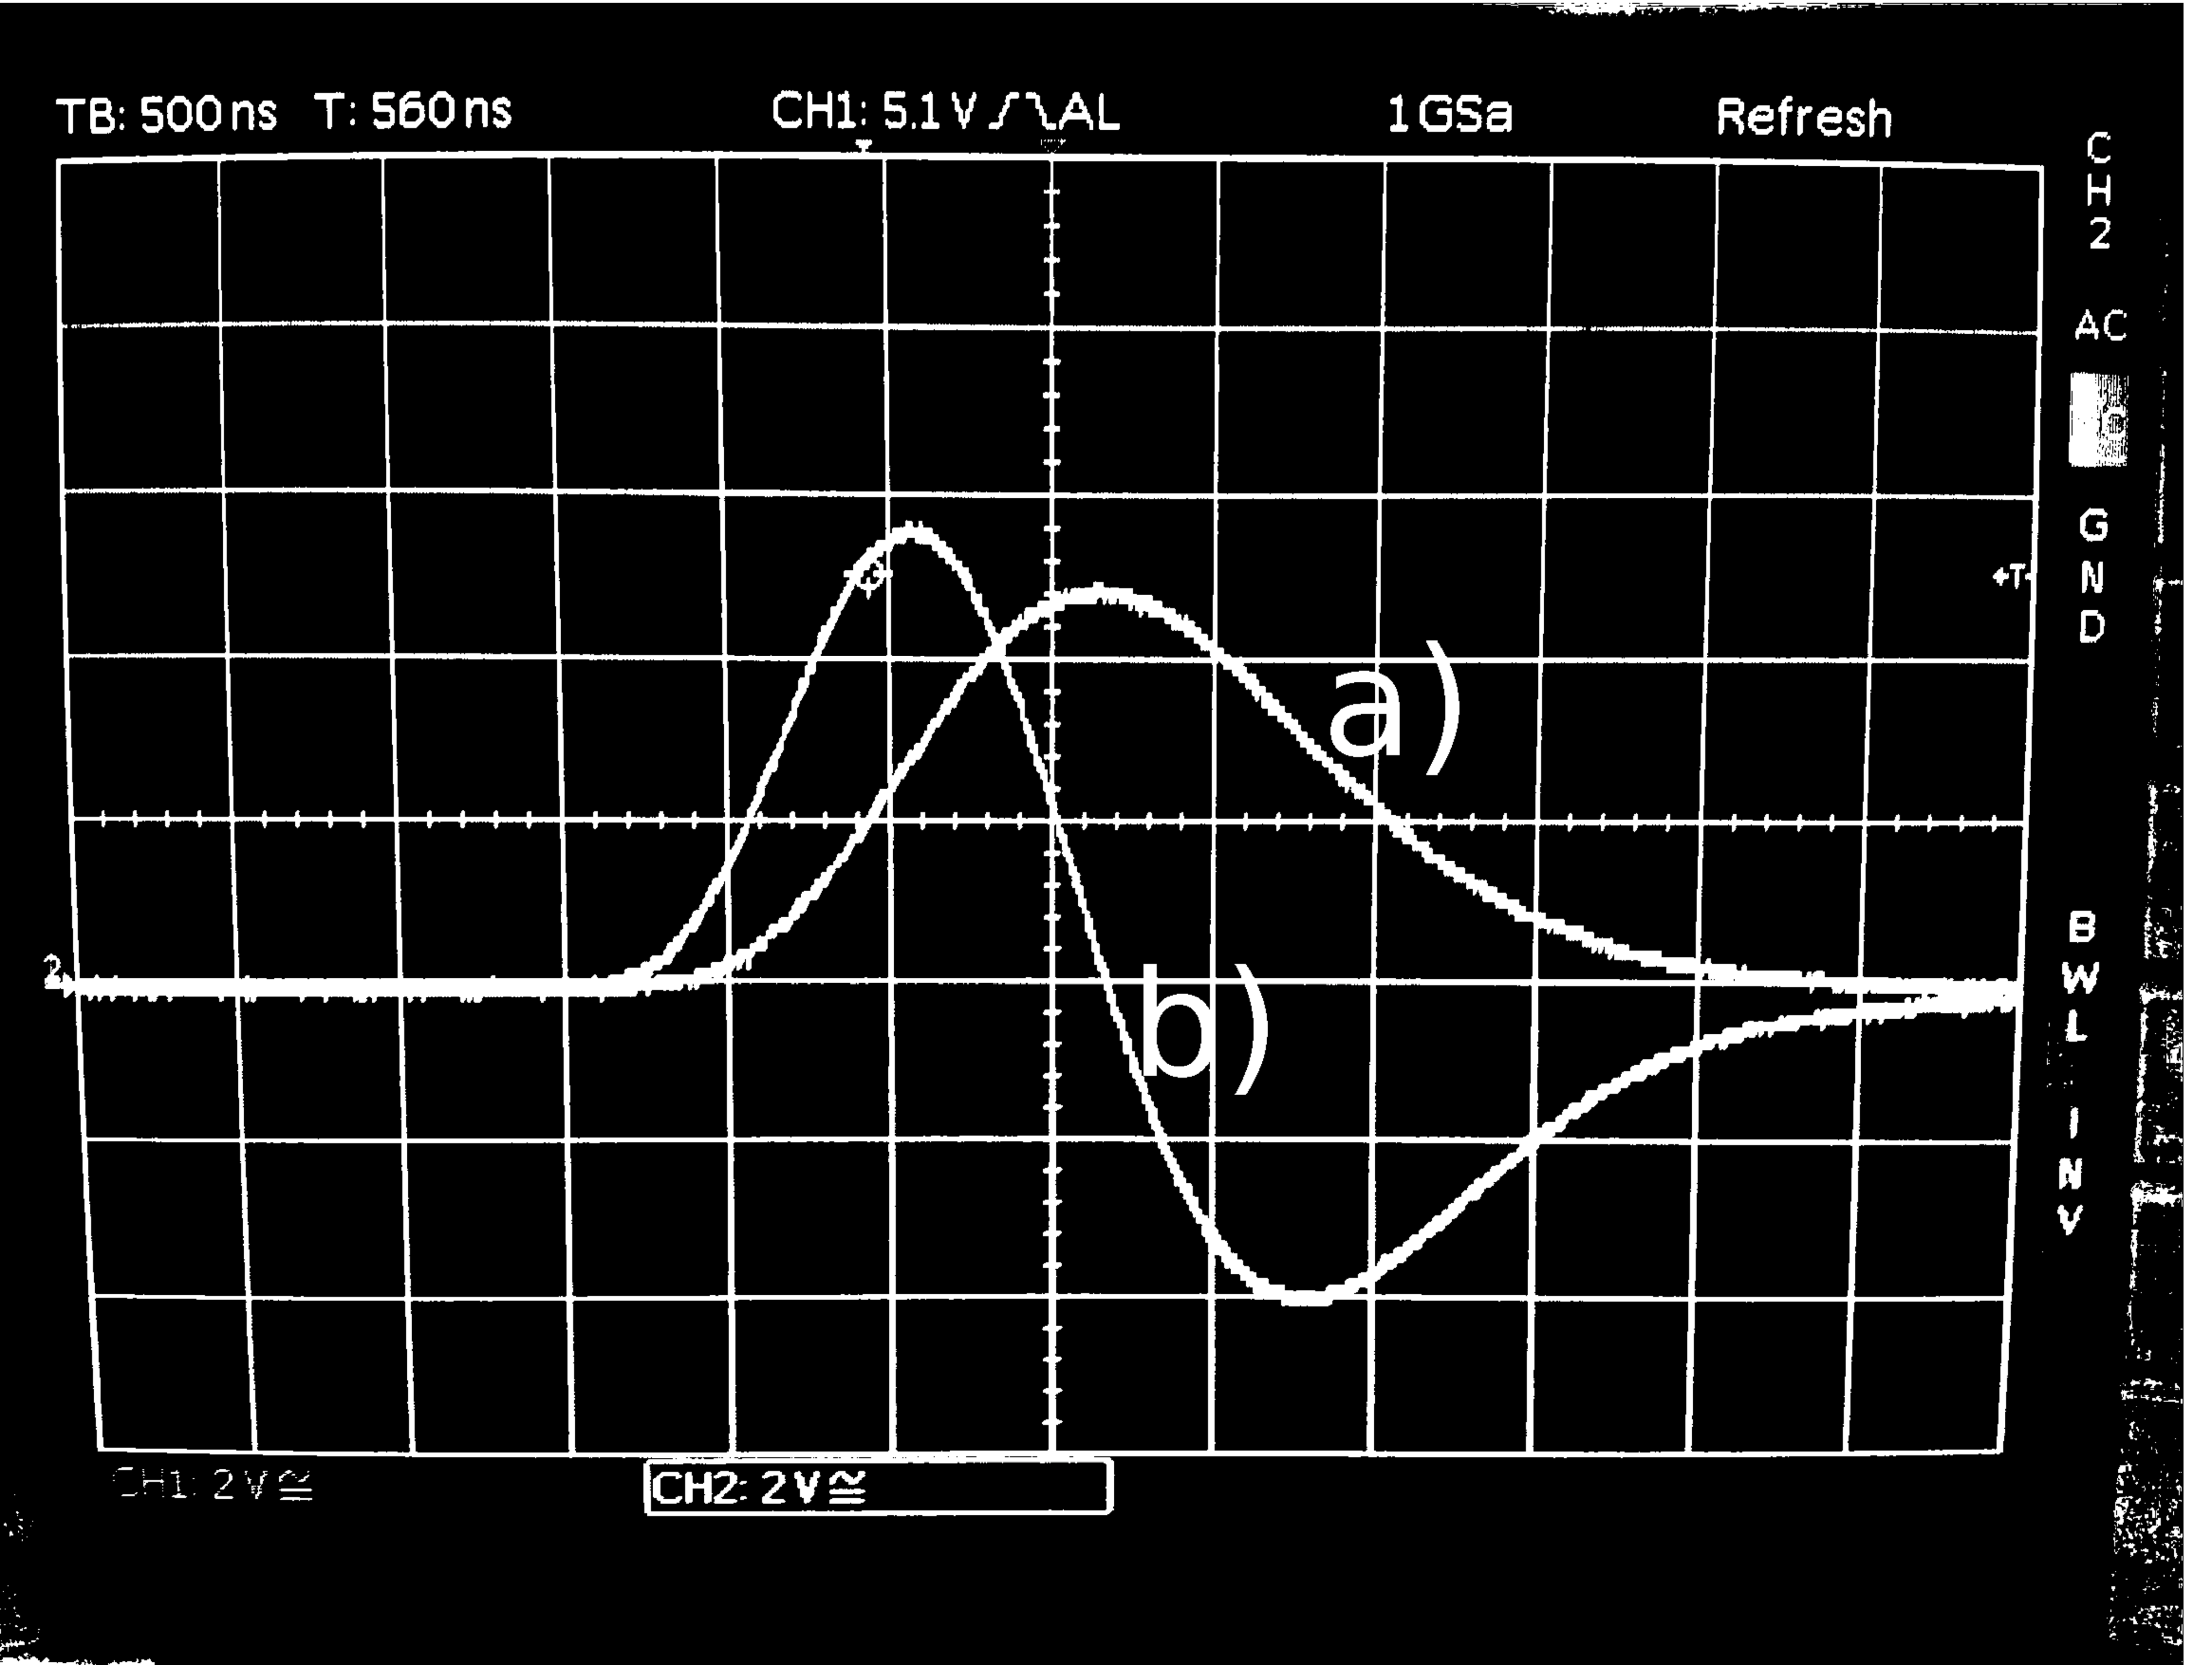
\includegraphics[width=0.8\linewidth]{figures/uni_bipolar2}
    \captionof{figure}{Oscillscope: a) refers to the unipolar channel and b) to 
the bipolar channel.}
  \end{minipage}
  \hfill
  \begin{minipage}[b]{0.49\textwidth}
    \centering
 \begin{tabular}{|l|l|}
     \hline
    course grain & 100\\
    gain    &   10.0 \\
    sharpening time &   0.5 \\
    sample & position 1\\
    PM & Right Side\\
    output & unipolar MCA\\
           & bipolar delay\\
     BLR & AFJ \\
     +/- & Pos \\
     delay & out\\
     \hline
\end{tabular}
\label{tab:config}
  \captionof{table}{Configuration of MA, MCA in measurement 2.1.1.}
    \end{minipage}
\end{minipage}

\subsubsection{Measuring the full energy spectrum}
\label{ssub:Measuring the full energy spectrum}
We increased the gain to 8.6 and the coarse gain to 200 of the MA, such that a observed spectrum 
was distributed of the entire range of bins, in order to be able to decide which detector and position would
be suitable. See Table~\ref{tab:config2} for our configuration of the setup. See
Figure~\ref{fig:measure2.1} for the figures of the measurement 2.1.
\begin{table}[htp]
    \begin{tabular}{|l|l|l||l|l|l|}
        \hline
        2.1a) & Positions:  & Pos1         & 2.1b) & Positions:  & Pos1\\
              & PM          & right        &       & PM          & left \\
              & Time        & $360\pm1$sec &       & Time        & $380\pm1$sec \\
        \hline 
        2.1c) & Positions:  & Pos2         & 2.1d) & Positions:  & Pos2         \\
              & PM          & right        &       & PM          & left \\
              & Time        & $402\pm1$sec &       & Time        & $368\pm1$sec \\
        \hline 
        2.1e) & Positions:  & Pos2         \\
              & PM          & left \\
              & Time        & $360\pm1$sec \\
    \cline{1-3}
    \end{tabular}
  \caption{Configuration in measurement 2.1 of Position, PM and integration time.}
    \label{tab:config2}
\end{table}

\begin{figure}
    \begin{subfigure}[b]{\picwidth}
        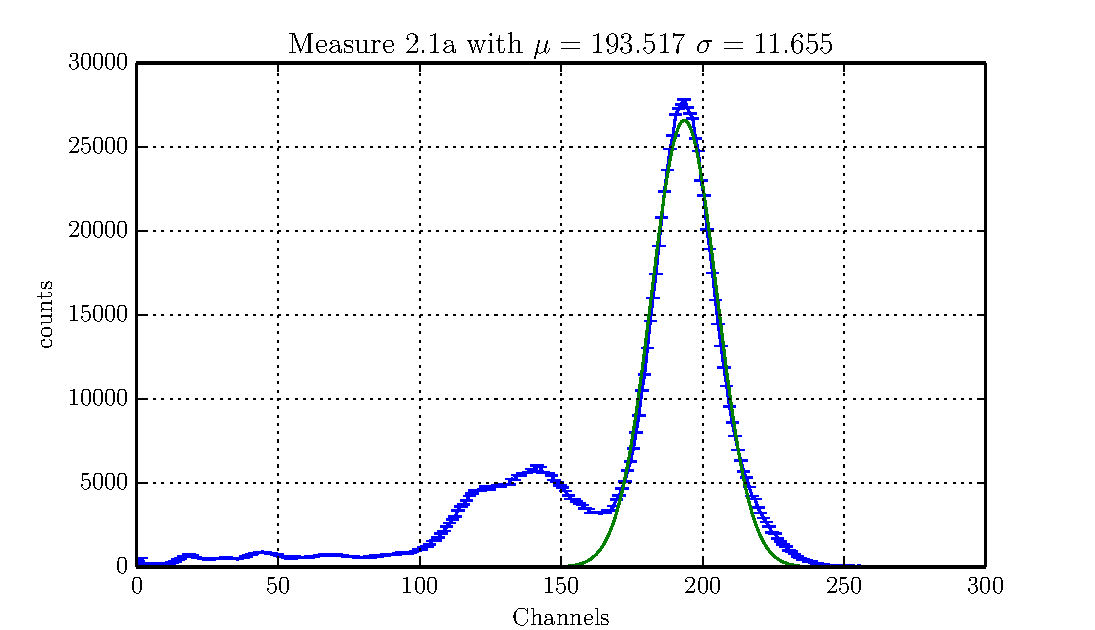
\includegraphics[width=\textwidth]{analysis/figures/plot2_1a}
        \caption{}
    \end{subfigure}\qquad
    \begin{subfigure}[b]{\picwidth}
        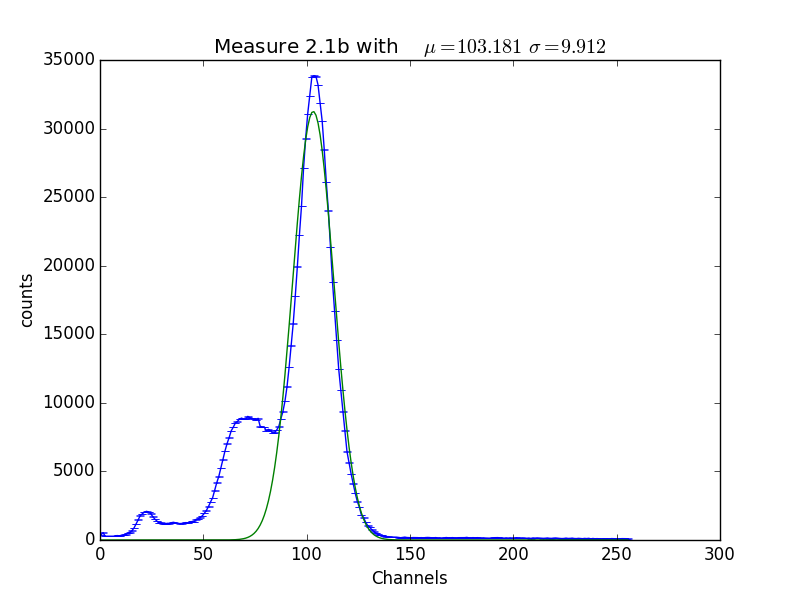
\includegraphics[width=\textwidth]{analysis/figures/plot2_1b}
        \caption{}
    \end{subfigure}
    \begin{subfigure}[b]{\picwidth}
        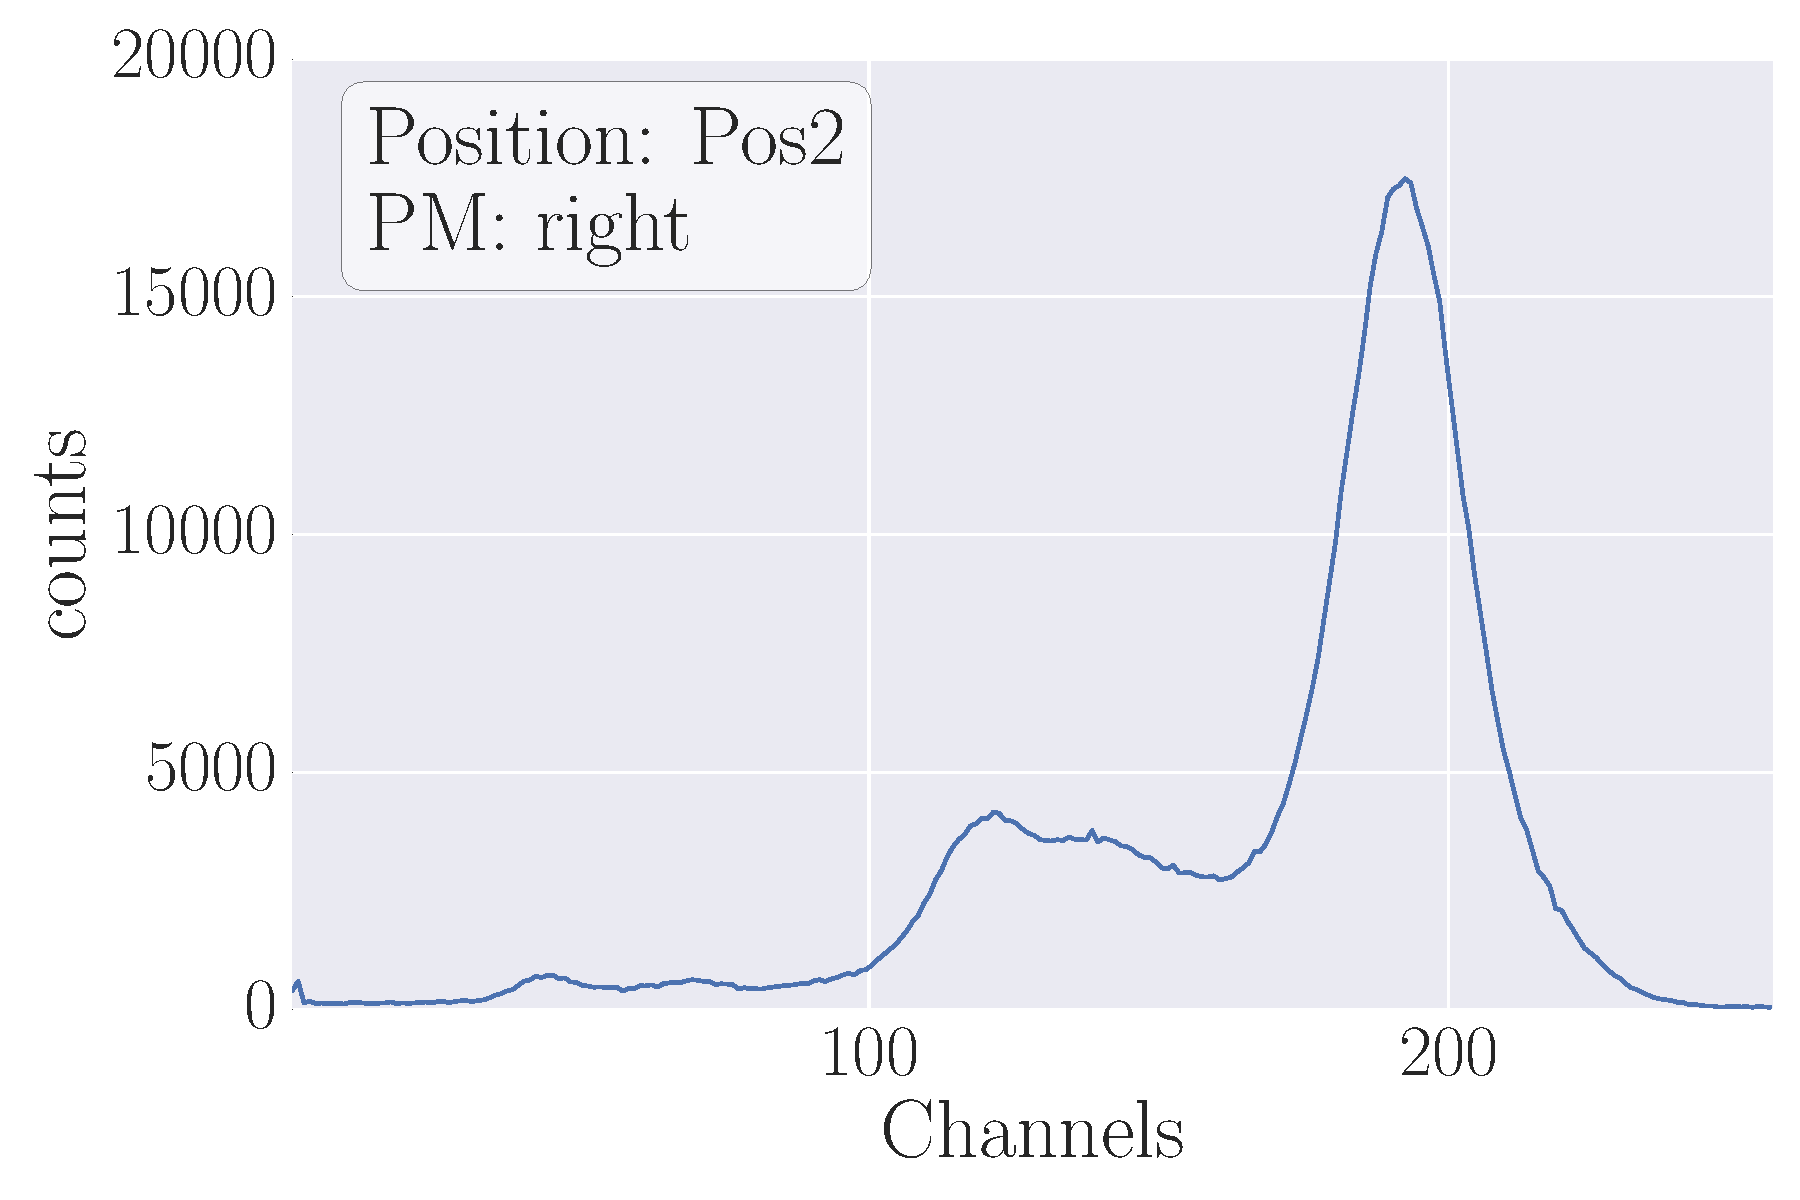
\includegraphics[width=\textwidth]{analysis/figures/plot2_1c}
        \caption{}
    \end{subfigure}
    \begin{subfigure}[b]{\picwidth}
        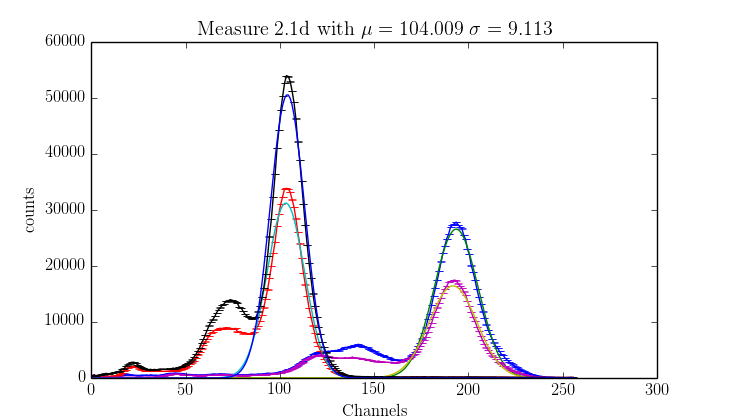
\includegraphics[width=\textwidth]{analysis/figures/plot2_1d}
        \caption{}
    \end{subfigure}
    \begin{subfigure}[b]{\picwidth}
        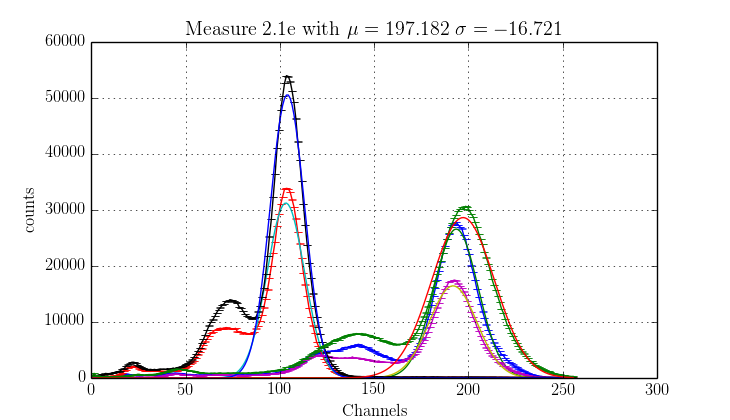
\includegraphics[width=\textwidth]{analysis/figures/plot2_1e}
        \caption{}
    \end{subfigure}
    \caption{Energy spectra with respect to the channels of the MCA, which we prescribed by
        measurements 2.1 (a) - (e).}
    \label{fig:measure2.1}
\end{figure}
\clearpage
\subsection{Measuring $\Delta t$ of coincidences}
\label{sub:measuring_delayed_coincidences}
\subsubsection{Setting the energy window}
\label{ssub:Setting the energy window}
From the results of the last chapter we have decided to chose position 1, which refers to measurements 2.1 a)
and 2.1 b). We only show the configuration of the successfull run with the right energy window chosen.
For the other configurations please see the appended records. For the the time delay we chose
$\Delta t = 140$ns.\\\\ 
 \begin{minipage}{\textwidth}
  \begin{minipage}[b]{0.49\textwidth}
   \begin{tabular}{|l|l|}
        \hline
       14.4 keV signal & right detector \\
       122 keV signal & left detector \\
       coarse gain & 200 \\
       gain & 8.6 \\
       Shaping time & $0.5\mu$s \\
        \hline
   \end{tabular}

  \captionof{table}{Configuration of MA1}
  \end{minipage}
  \hfill
  \begin{minipage}[b]{0.49\textwidth}
    \centering
   \begin{tabular}{|l|l|}
        \hline
       Lower Level & $4.75\pm0.05$ \\
       Upper Level & $3.72\pm0.05$ \\
       Delay & 1.0 (minimum possible) \\
        walk ADJ & $0.1 - 1.1\mu$s (NOR)  \\
       Pos Out & Linear Gate ``enable''\\
        \hline
   \end{tabular}
  \captionof{table}{Configuration of SCA1}
\end{minipage}
\end{minipage}
\begin{minipage}{\textwidth}
  \begin{minipage}[b]{0.49\textwidth}
   \begin{tabular}{|l|l|}
        \hline
       coarse gain & 500 \\
       gain & 8.6 \\
       Shaping time & $0.5\mu$s \\
       input & right detector \\ 
        delay & out \\
        \hline
   \end{tabular}

  \captionof{table}{Configuration of MA2}
  \end{minipage}
  \hfill
  \begin{minipage}[b]{0.49\textwidth}
    \centering
   \begin{tabular}{|l|l|}
        \hline
       Lower Level & $2.02\pm0.05$ \\
       Upper Level & $3.04\pm0.05$ \\
       Delay & 1.0 (minimum possible) \\
        walk ADJ & $0.1 - 1.1\mu$s (NOR)  \\
       Pos Out & Linear Gate ``enable''\\
        \hline
   \end{tabular}
  \captionof{table}{Configuration of SCA2}
\end{minipage}
\end{minipage}
\clearpage
\subsubsection{Delayed coincidences}
The measurement ran about 14 hours over night. See Figure~\ref{fig:4_1} for the visualization.
\label{ssub:Conduction of the experiment over night}

\begin{figure}[htpb]
    \centering
    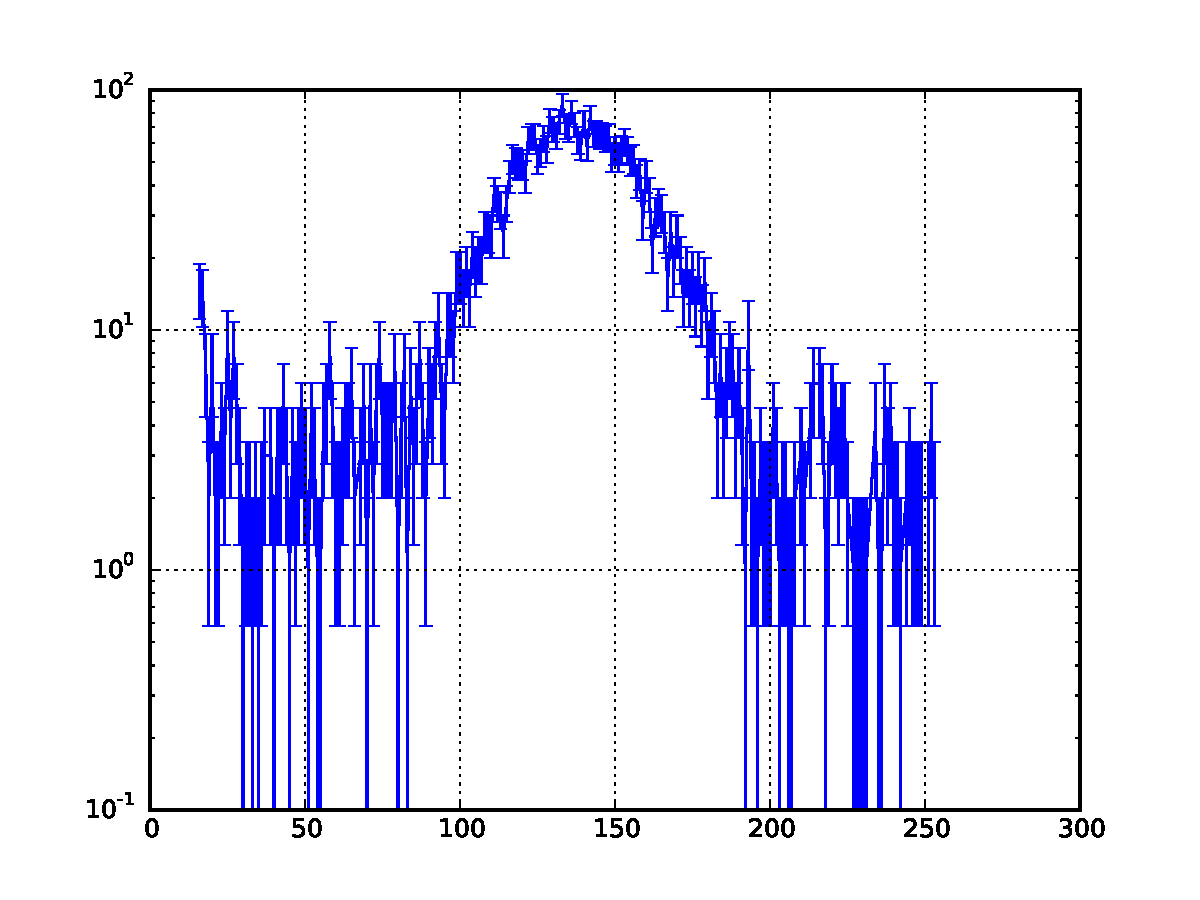
\includegraphics[width=1.0\linewidth]{analysis/figures/plot4_1}
    \caption{Measurement 4.1: You will notice that the shape
        of the peak looks gaussian, which is rather unexpected. However
        further analysis show, that the peak is not symmetric and hence the left 
        side will be fitted against a exponential curve, while the origin of the
        right side is the background, which will be analyzed in the next section.
        The errors which are visualized here are approximated by $S_{N_i} = \sqrt{N_i}$.}
    \label{fig:4_1}
\end{figure}
\clearpage
\subsubsection{Random coicidences}
\label{ssub:Random coicidences}
For measuring the background we used the same configuration as before, except of the TAC-input:
\begin{itemize}
    \item TAC Start: SCA2, triggered by the 14.4 keV Peak, delayed with $\Delta t = 48$ns
    \item TAC Stop: SCA1, triggered by 122 keV (no delay)
\end{itemize}
A first approach with $\Delta t = 16$ns failed, since we observed a clear peak in low channels in contrary
to an expected equally distributed signal. After changing to $\Delta t=48$ns we observe a clear
background noise signal, which you can see in Figure~\ref{fig:5_1}.
\begin{figure}[htpb]
    \centering
    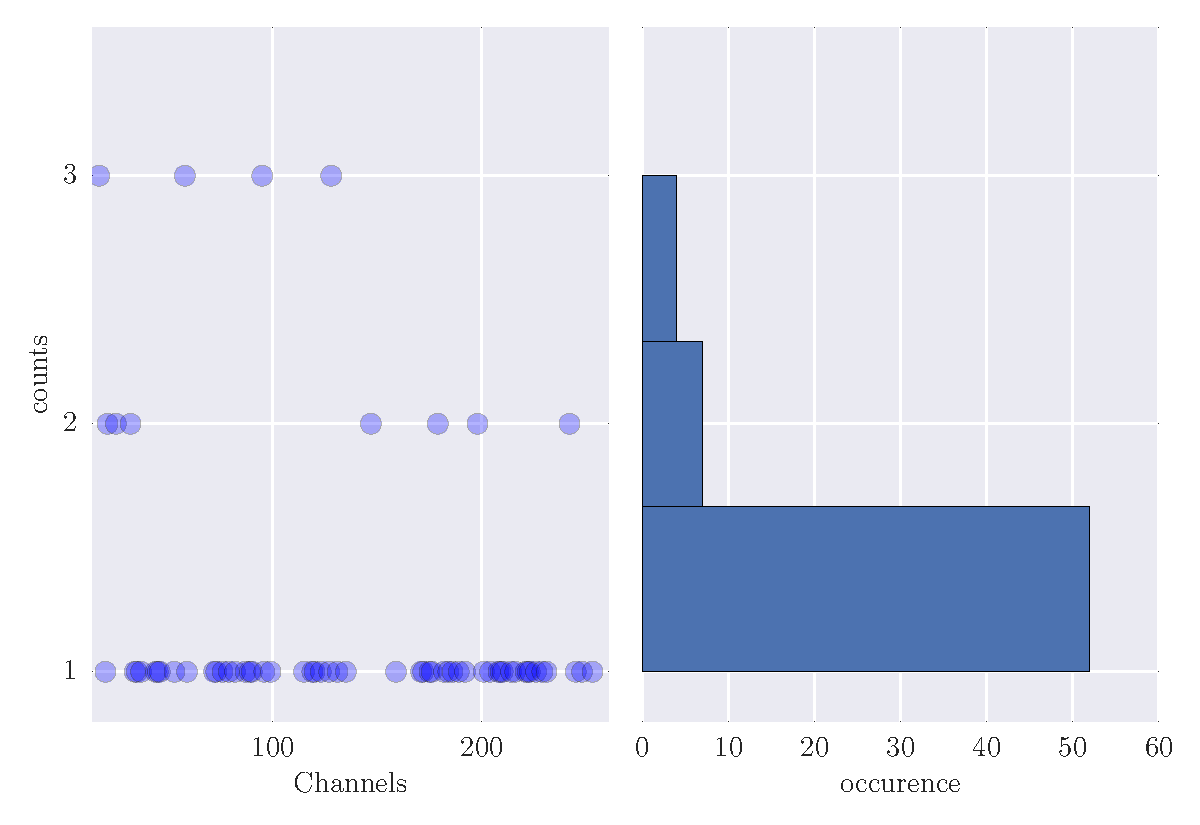
\includegraphics[width=1.0\linewidth]{analysis/figures/plot5_1_hist}
    \caption{Measurement 5.1: Random coincidences and their histogram.}
    \label{fig:5_1}
\end{figure}

\clearpage
\subsection{Calibration of TAC-MCA Signal}
\label{sub:calibration_of_tac_mca_signal}
\begin{figure}[htpb]
    \centering
    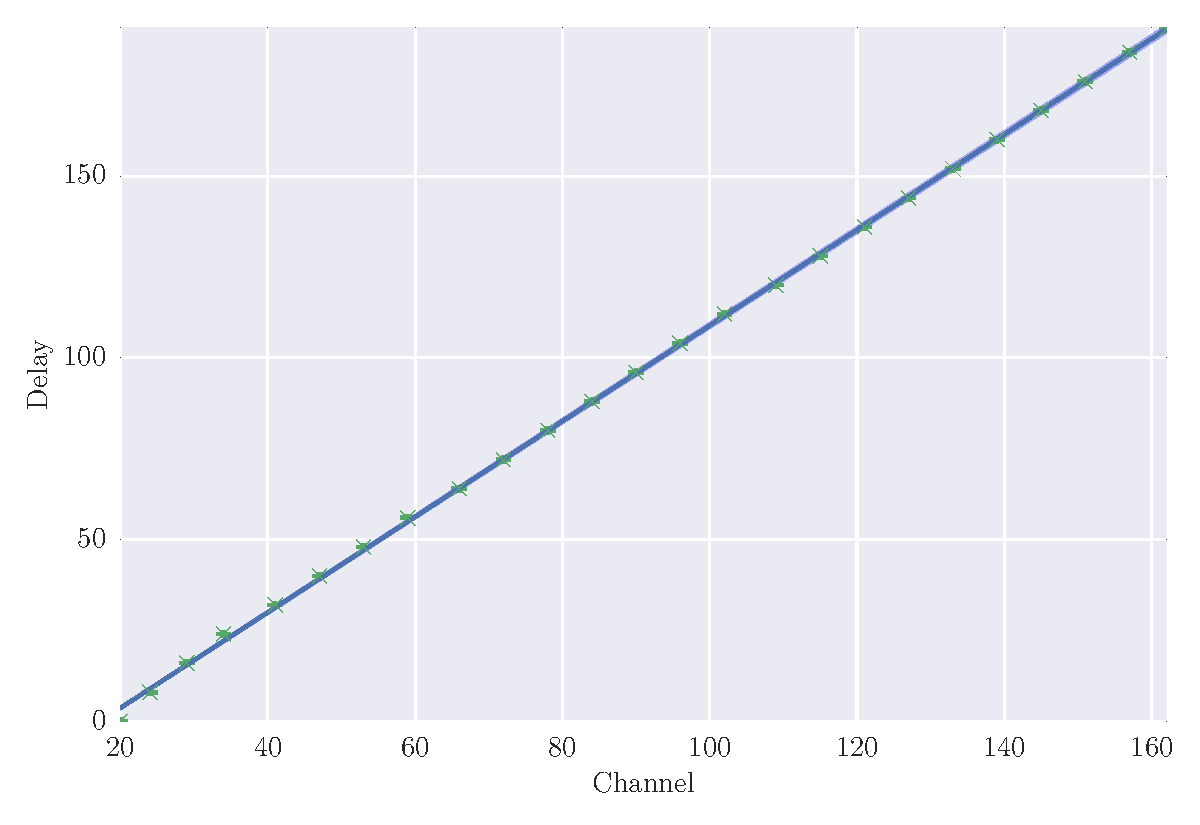
\includegraphics[width=0.7\linewidth]{analysis/figures/plot7}
    \caption{Calibration of the TAC-MCA Signal.}
    \label{fig:plot7}
\end{figure}
\begin{figure}[htpb]
    \centering
    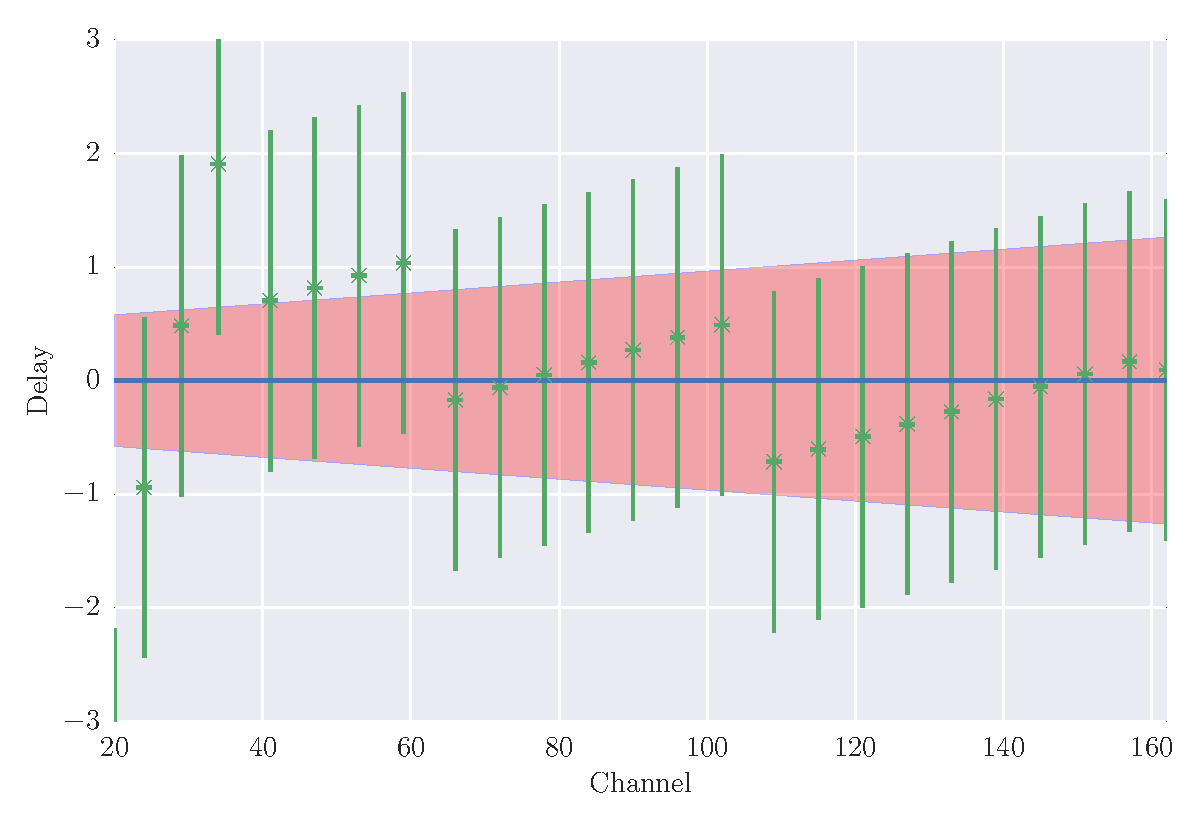
\includegraphics[width=0.7\linewidth]{analysis/figures/plot7b}
    \caption{Calibration of the TAC-MCA Signal.}
    \label{fig:plot7}
\end{figure}




\section{Conclusion}
In the first part of the experiment, we basically obtained one 
central results: The approximated band gap energy $E_g$ for germanium 
and silicon. Our measured values lie at 
\begin{align}
    E_{g, \mathrm{Si}} &= (1.14 \pm 0.05) \,\mathrm{eV} \\
    E_{g, \mathrm{Ge}} &= (0.69 \pm 0.03) \,\mathrm{eV}
\end{align}
Both values cover the literature values within one standard deviation.
This accuracy was a rather surprising result to us, as we expected the 
applied method to be of a much lower certainty. 

The values measured in the Haynes \& Shockley experiment 
are displayed in the table~\ref{tab:conc_h_s} below:
\renewcommand{\arraystretch}{1.5}
\begin{table}[H]
    \centering
    \caption{
        Results of the Haynes \& Shockley experiment, variating the 
        acceleration voltage or the distance between creating the 
        cloud of free charge and measuring it. The errors correspond 
        to propagated errors of fitting not including systematical ones 
        and are thus underestimated. 
        }
	\begin{tabular}{|p{4cm}|p{3cm}|p{3cm}|p{3cm}|}
		\hline
		\rowcolor{tabcolor}
		Parameter           & $U = \text{const.}$   & $d = \text{const.}$   & Literature~\cite{staatsexamen} \\ 
        \hline
        mobility $\mu_n$    & $2640 \pm 130$        & $3000 \pm 120$        & $3900$     \\
        life time $\tau_n$  & $6.7 \pm 1.0$         & $1.6 \pm 0.5$         & $45 \pm 2$ \\
        diffusion const. $D_n$ & $140 \pm 20$      & $130 \pm 20$          & $101$     \\
		\hline
	\end{tabular}
    \label{tab:conc_h_s}
\end{table}
For both the electron mobility and diffusion constant we observe agreement in the 
order of magnitude between our results and the given literature values. The 
errors are underestimated due to not including systematical errors in the calculation. 
Other the shortcomings of the electronics (which we experienced in terms 
of loosing the signal), it is clear that the experiment does not allow the 
measurement of these constants in a perfect crystal. This is especially 
true for the life time, which is one order of magnitude smaller then the 
accepted value for germanium. 

Examination of the two semiconductors Si and CdTe gave an insight into the 
characteristics that allow for the usage as detectors for ionizing 
radiation. The central result is the superiority of heavier materials
(here represented by CdTe) over light ones (Si) when the registration of as 
many events as possible is key. The quantitative result, 
the ratio of absorption coefficients has been estimated to be
\begin{align}
    \mathrm{\frac{Abs_{Si}}{Abs_{CdTe}}}(59.5\, \mathrm{keV}) &= (3.51 \pm 0.07) \\
    \mathrm{\frac{Abs_{Si}}{Abs_{CdTe}}}(122.06\, \mathrm{keV}) &= (1.16 \pm 0.08)\\ 
    \mathrm{\frac{Abs_{Si}}{Abs_{CdTe}}}(136.47\, \mathrm{keV}) &= (1.9 \pm 0.6) \, ,
\end{align}
agreeing with the literature values in order of magnitude. The errors 
are those obtained by numerical calculation and do not include 
systematical errors, such as impurities or errors induced by the electronics. 
With one setup and the two possible semiconductors as detectors, one 
would thus need to measure 30 to 60 times as long with the Si semiconductor 
to obtain the same number of counts and thus the same statistical error. 
As a second, somewhat less striking result, we calculated the 
relative energy resolution (RER). The main result here is the increasing 
resolution with increasing energy: The resolution at 122 keV Co peak is 
twice the one at the 59.5 keV Am peak for both semiconductors.  

All three experiments resulted in a good introduction into semiconductor physics. 
Especially the Haynes and Shockley experiment, notwithstanding the disagreement in 
numerical results, gave a nice insight into models of the reality in semiconductors. 



\section{Bibliography}
\printbibliography[heading=subbibintoc]
\clearpage

\section{Appendix: Handwritten records of the experiment}
\label{sec:appendix}
    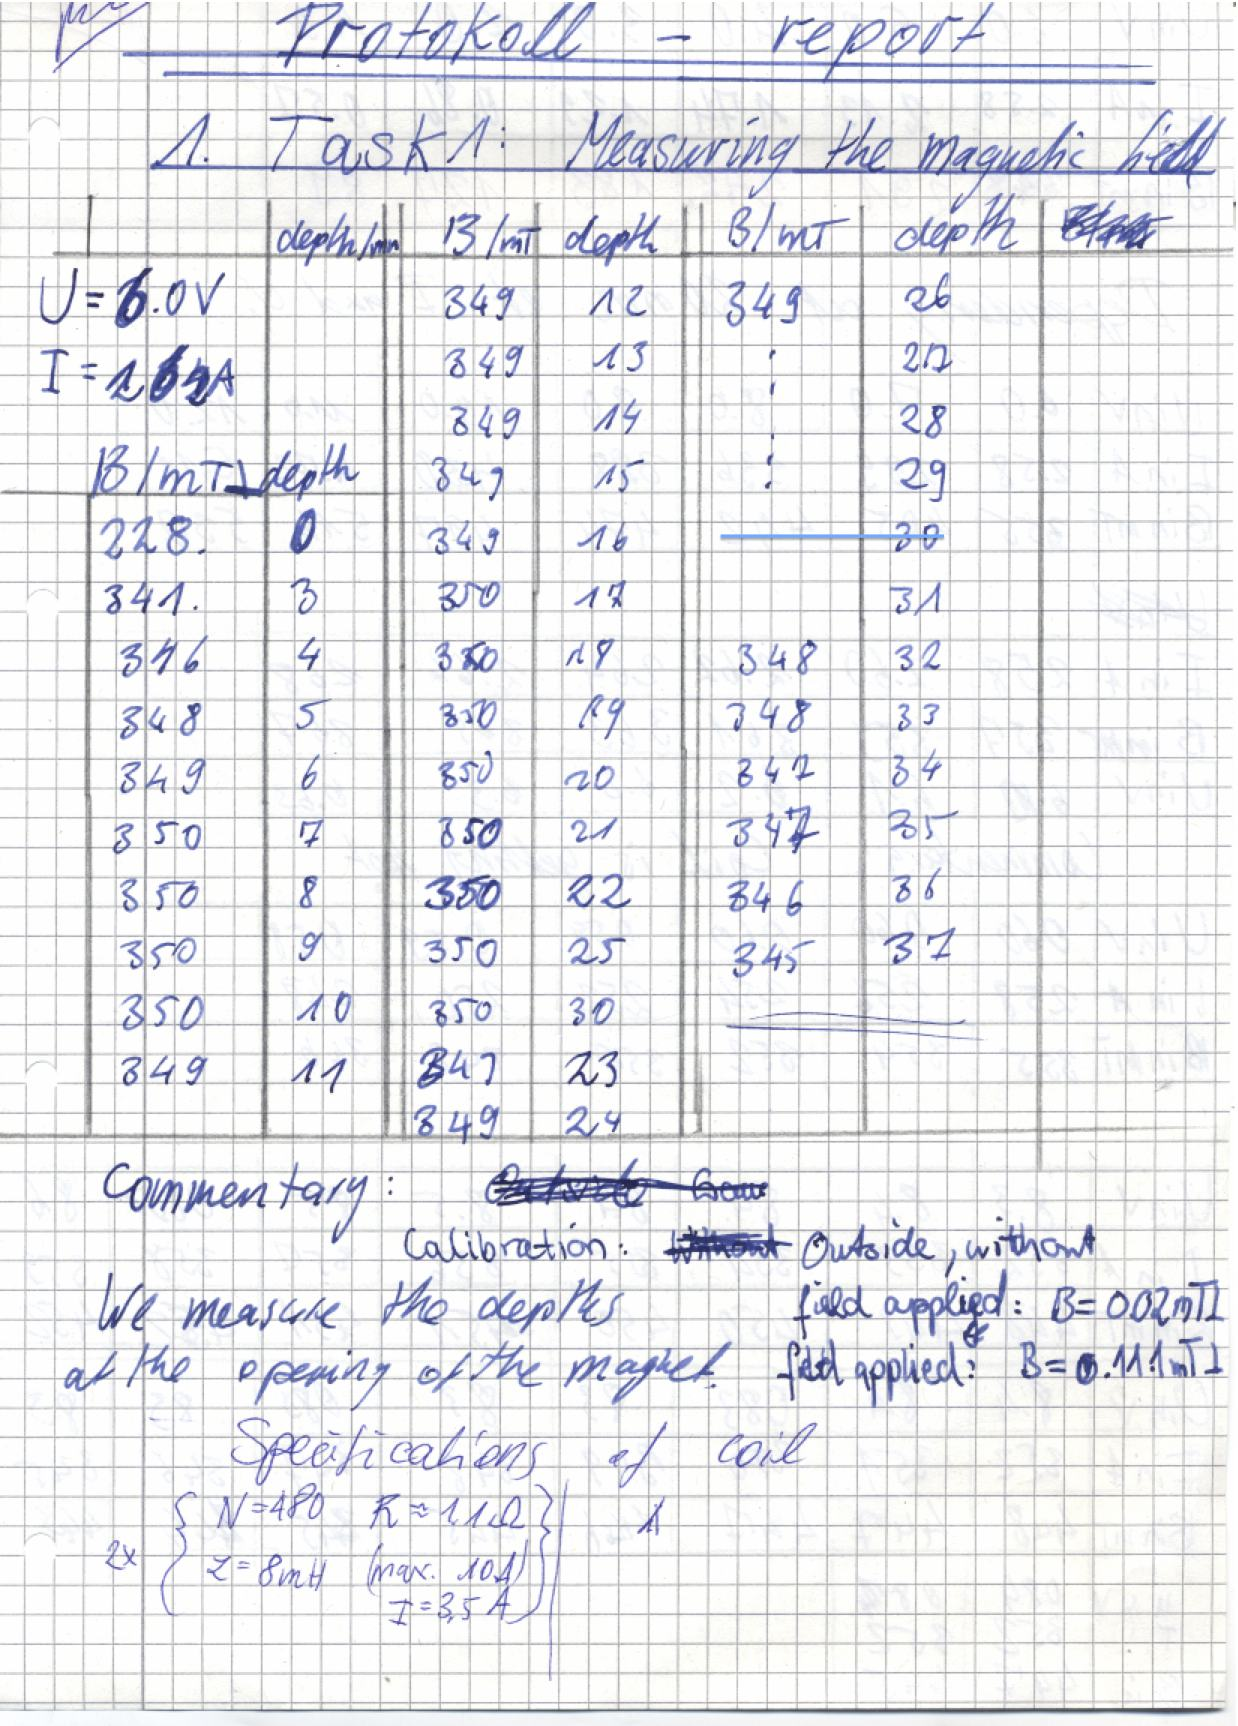
\includegraphics[width=\linewidth]{appendix/spin1.jpg}
\clearpage
    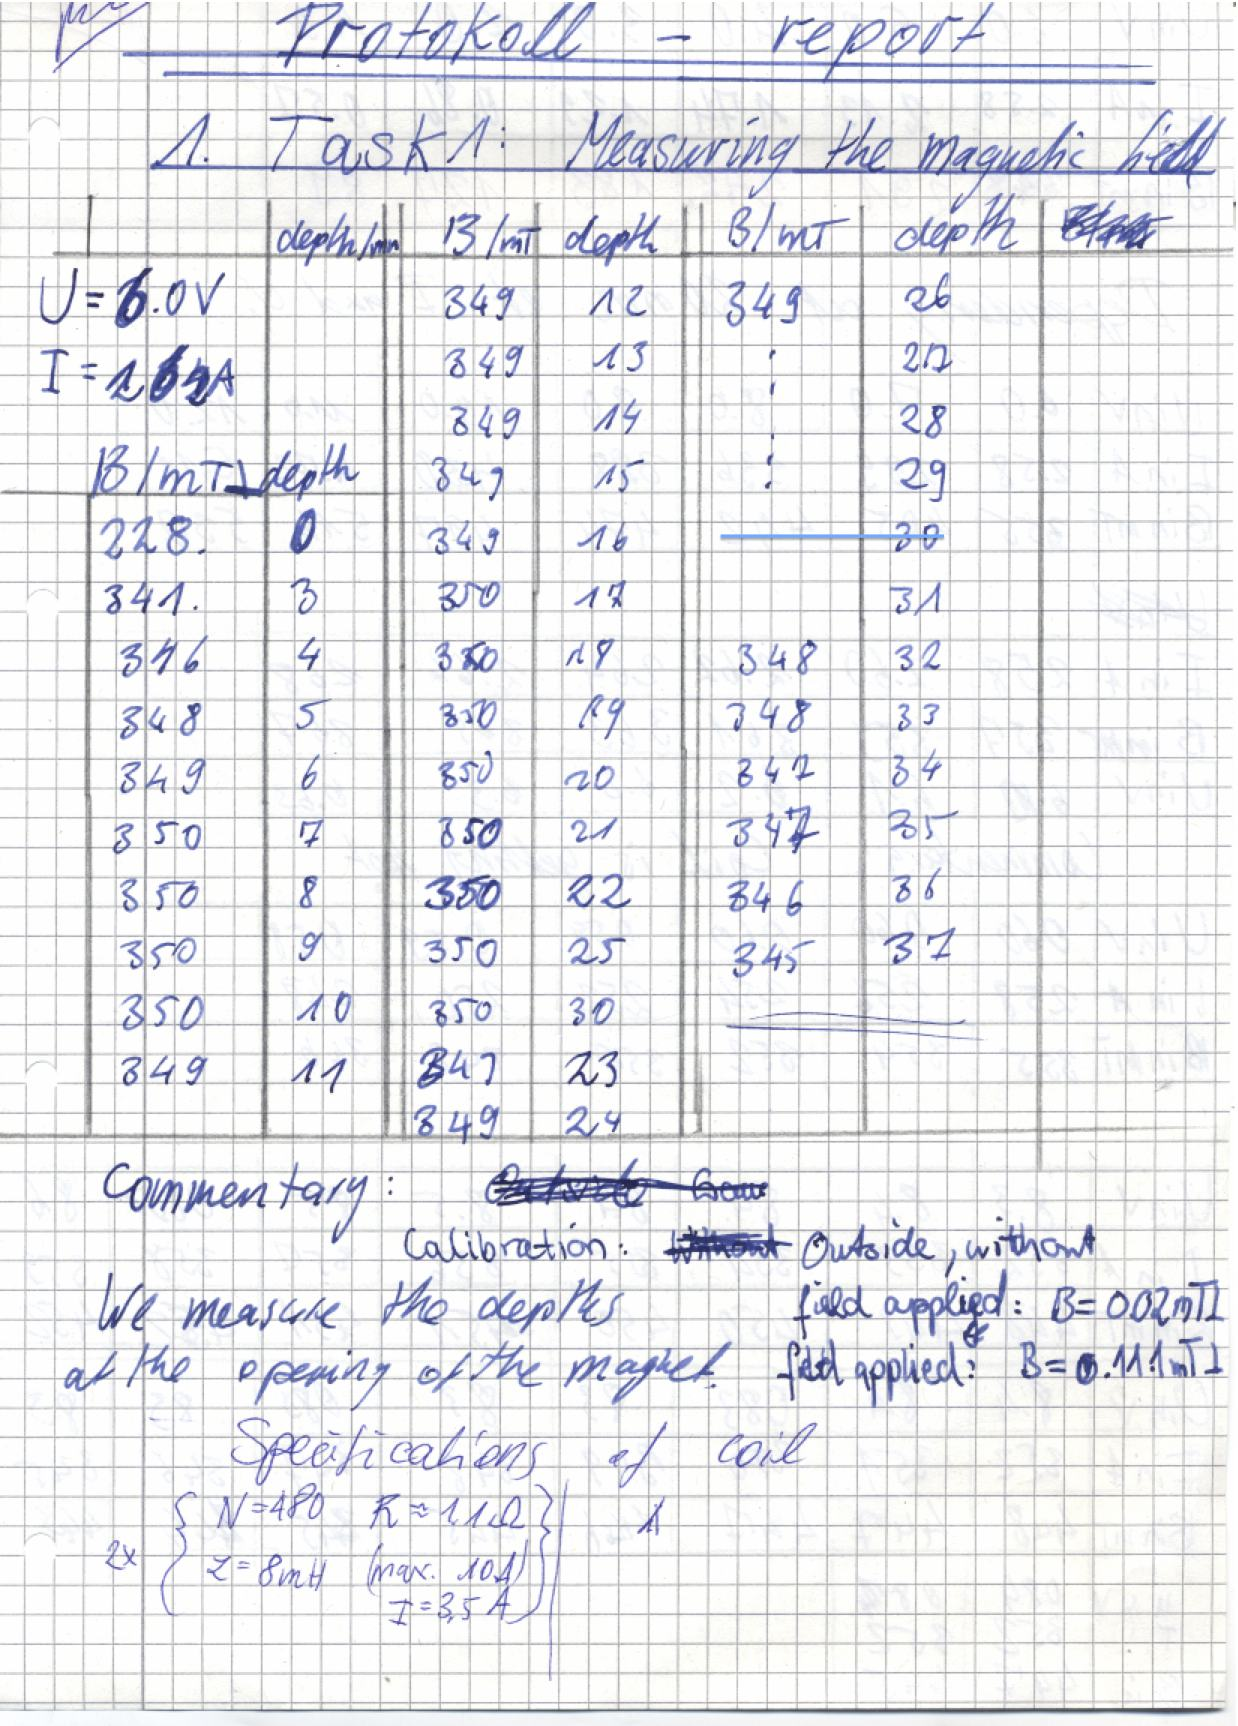
\includegraphics[width=\linewidth]{appendix/spin1.jpg}
\clearpage
    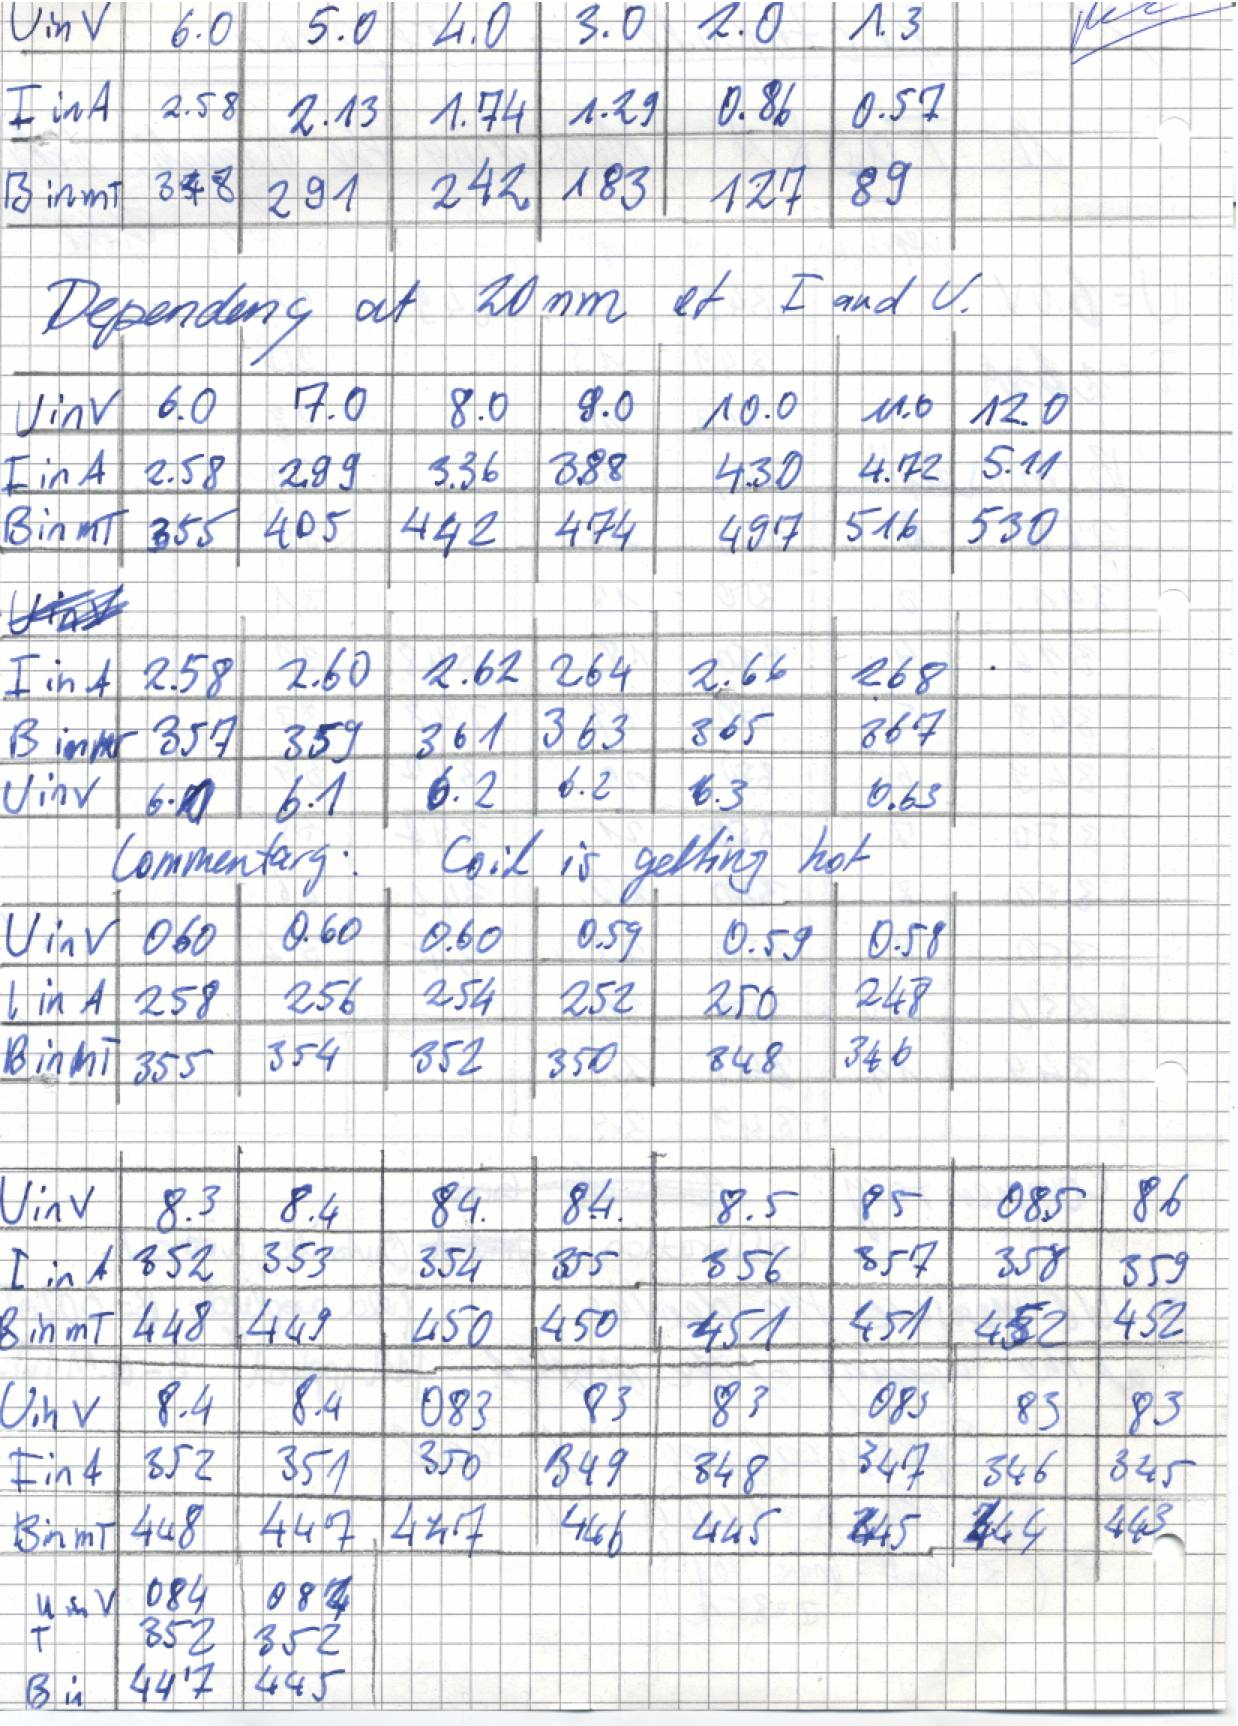
\includegraphics[width=\linewidth]{appendix/spin2.jpg}
\clearpage
    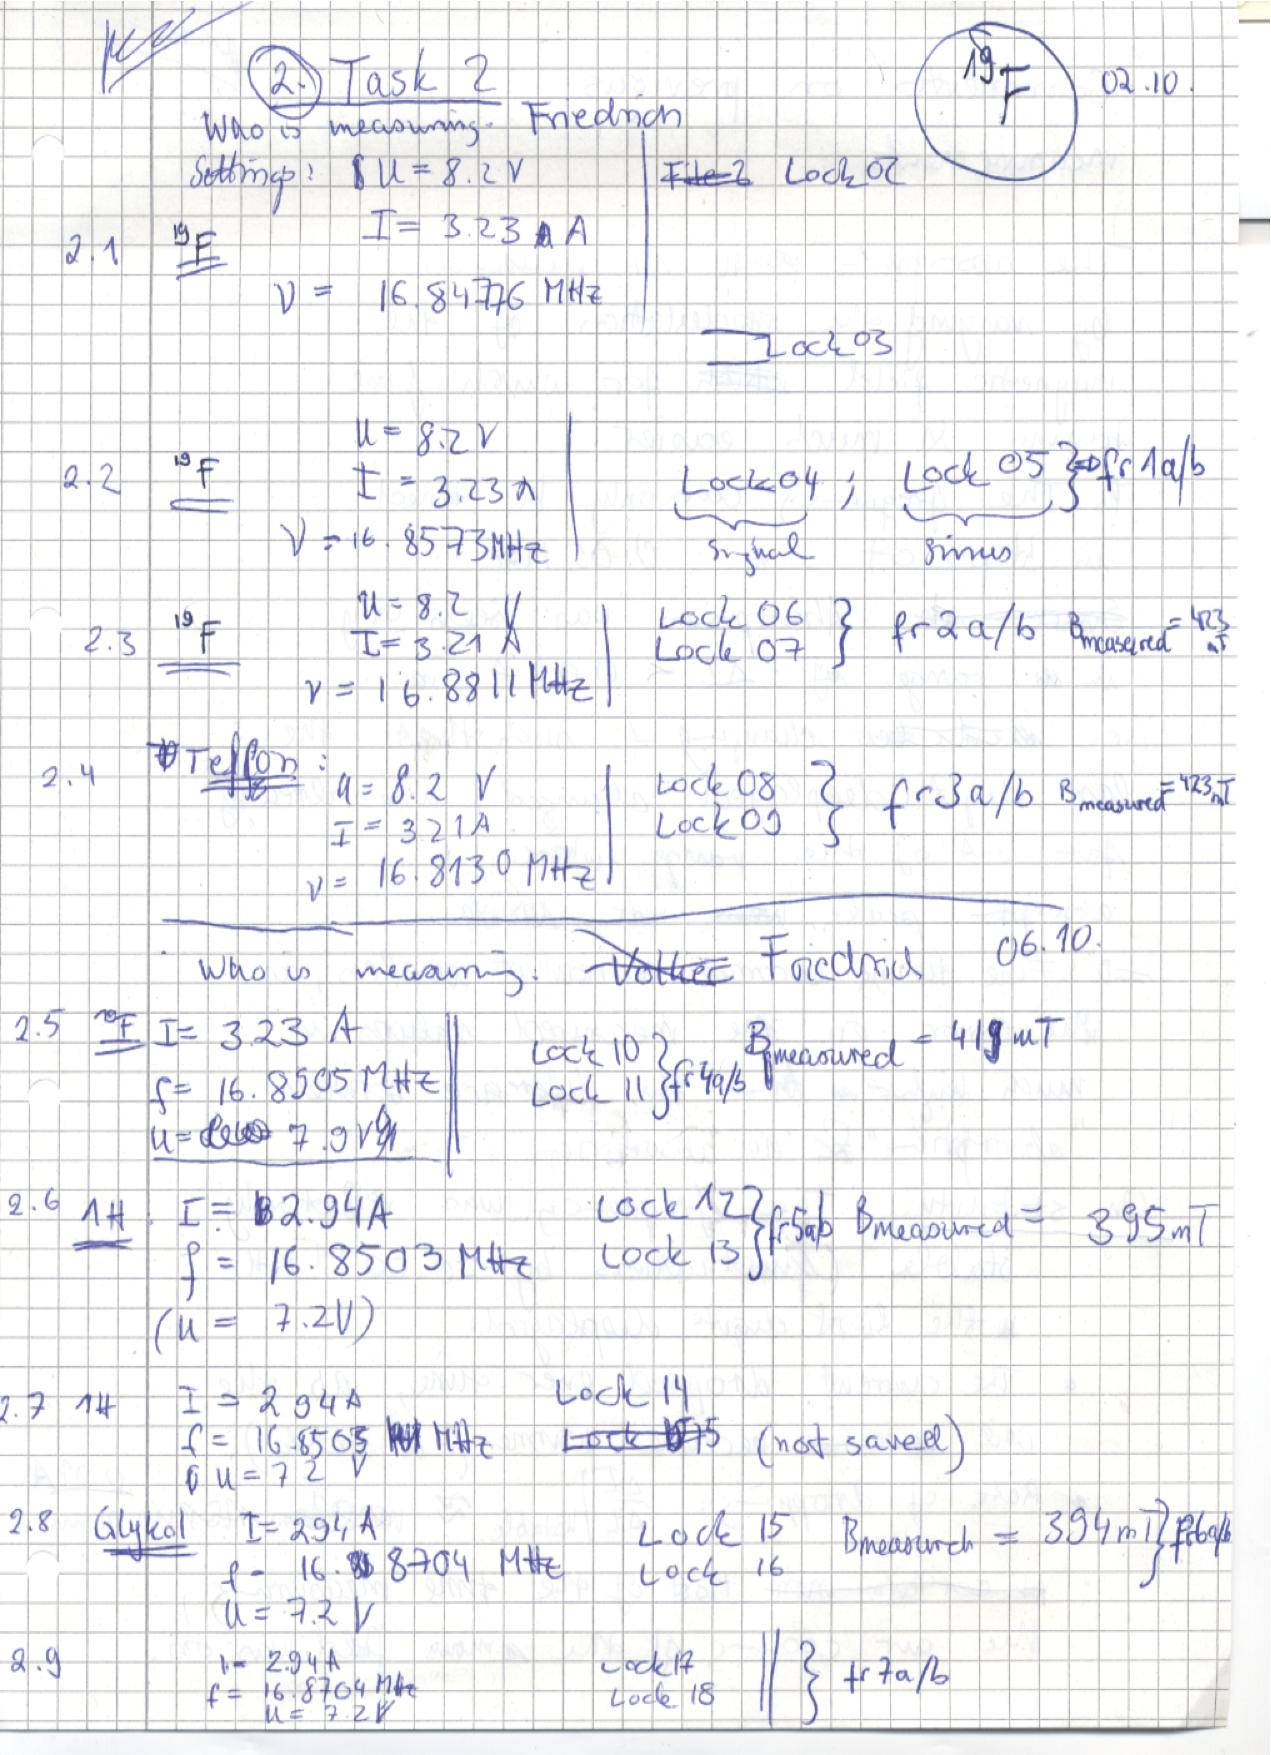
\includegraphics[width=\linewidth]{appendix/spin3.jpg}
\clearpage
    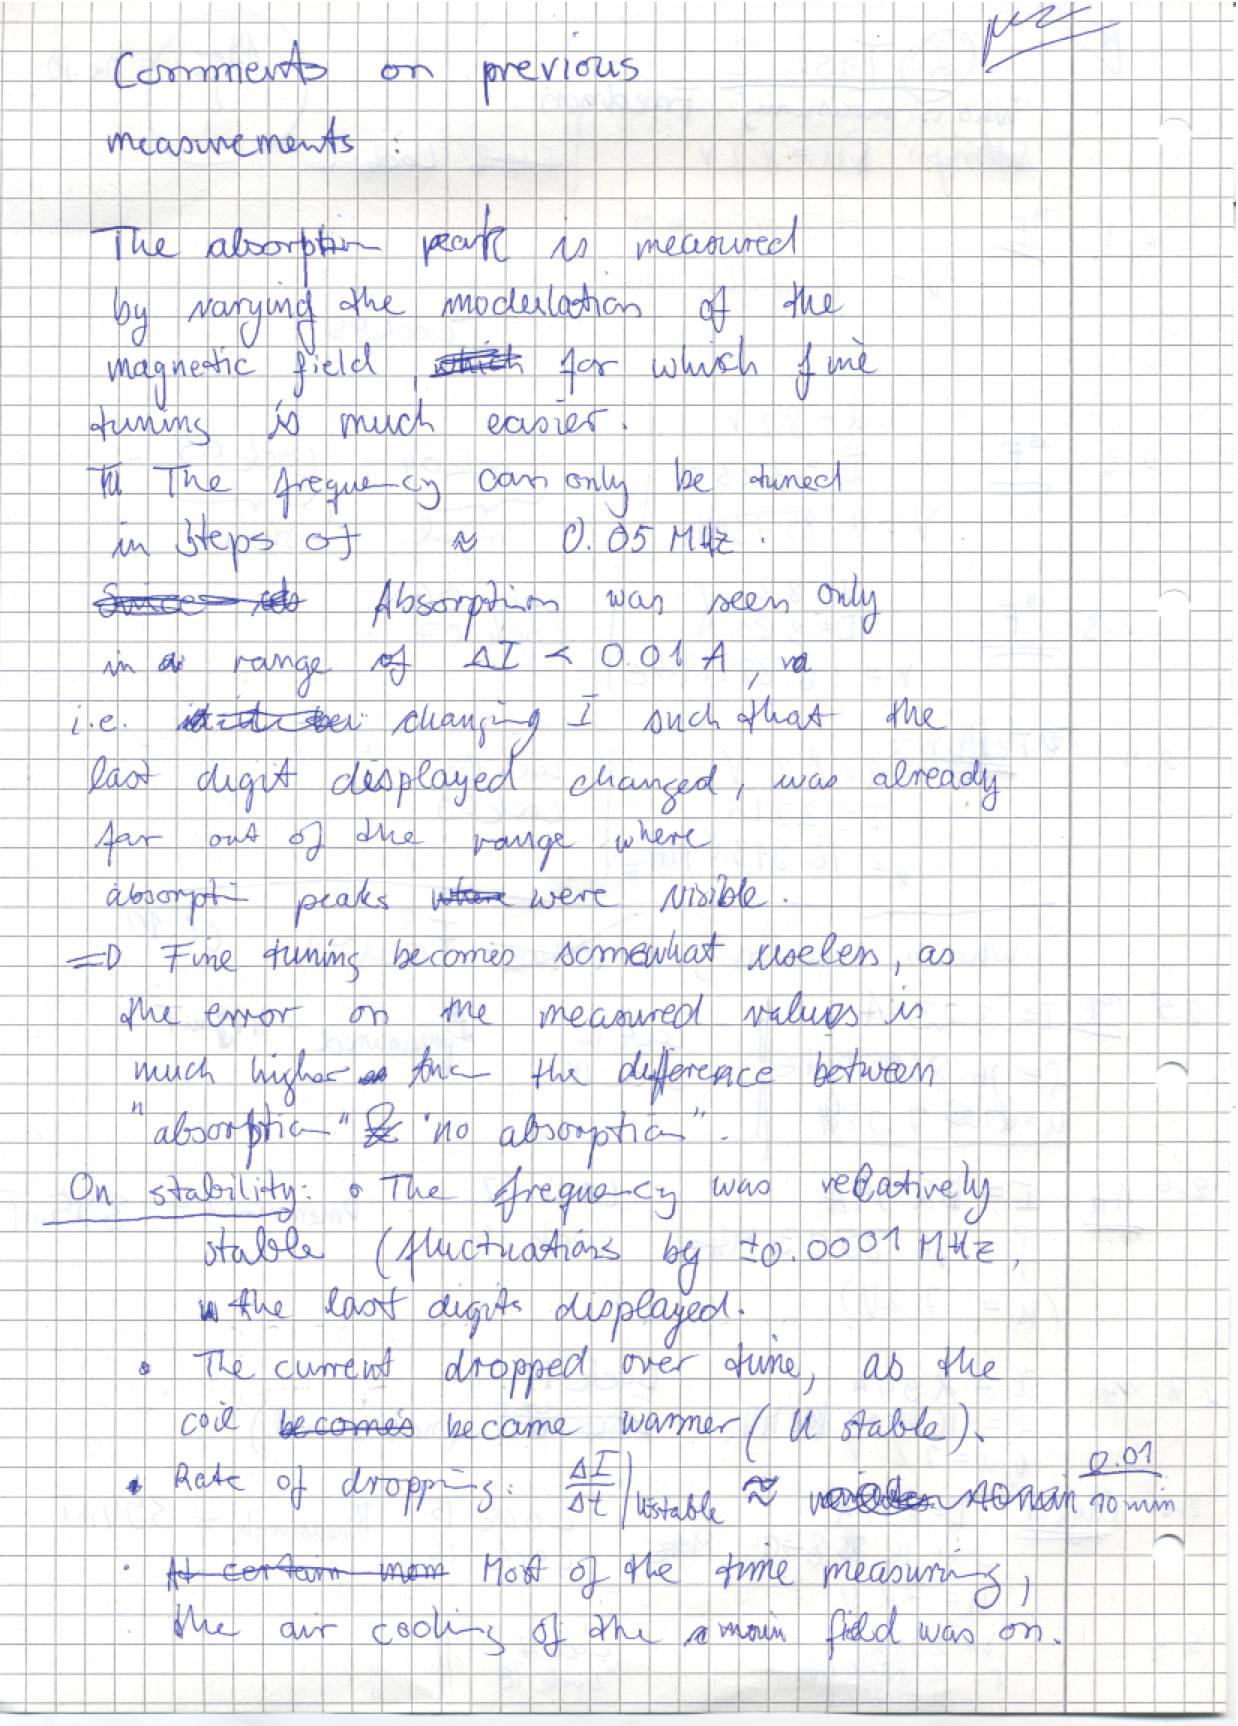
\includegraphics[width=\linewidth]{appendix/spin4.jpg}
\clearpage
    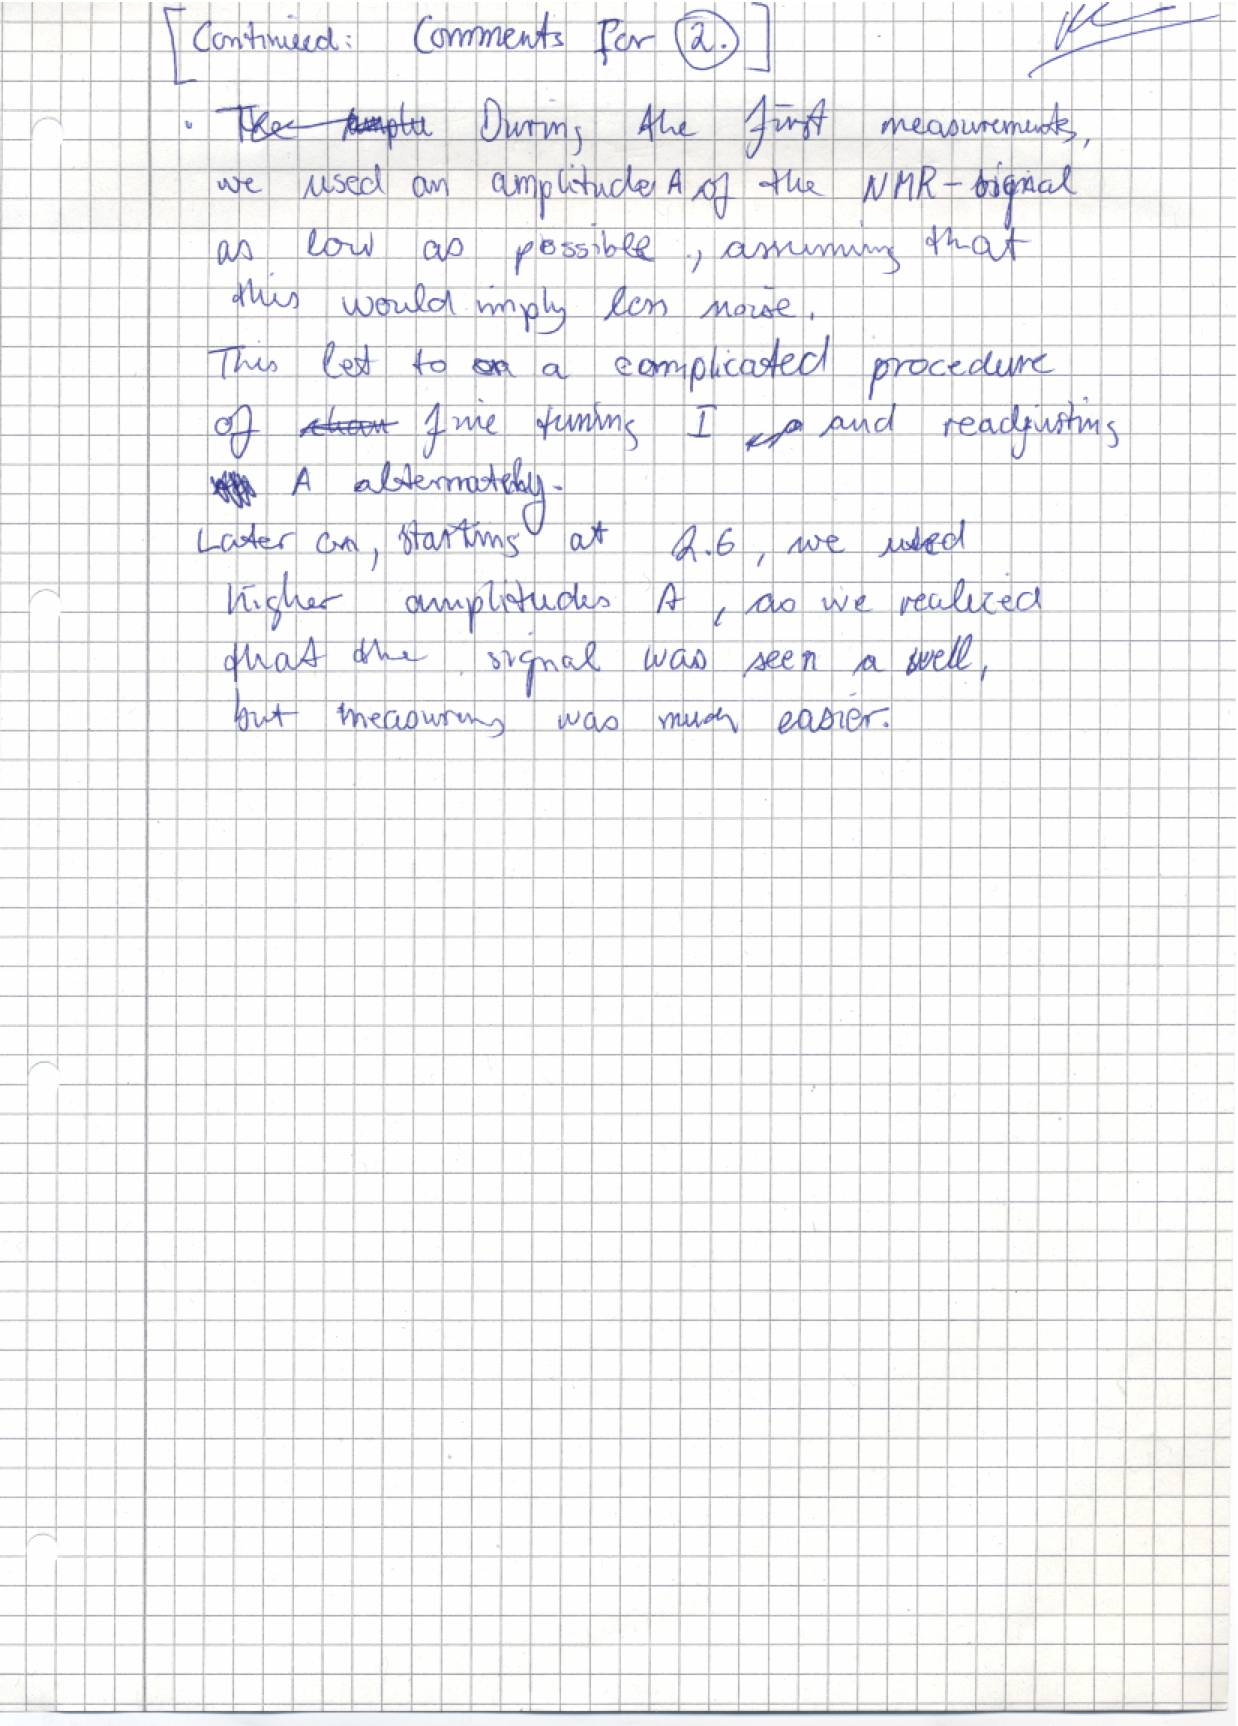
\includegraphics[width=\linewidth]{appendix/spin5.jpg}
\clearpage
    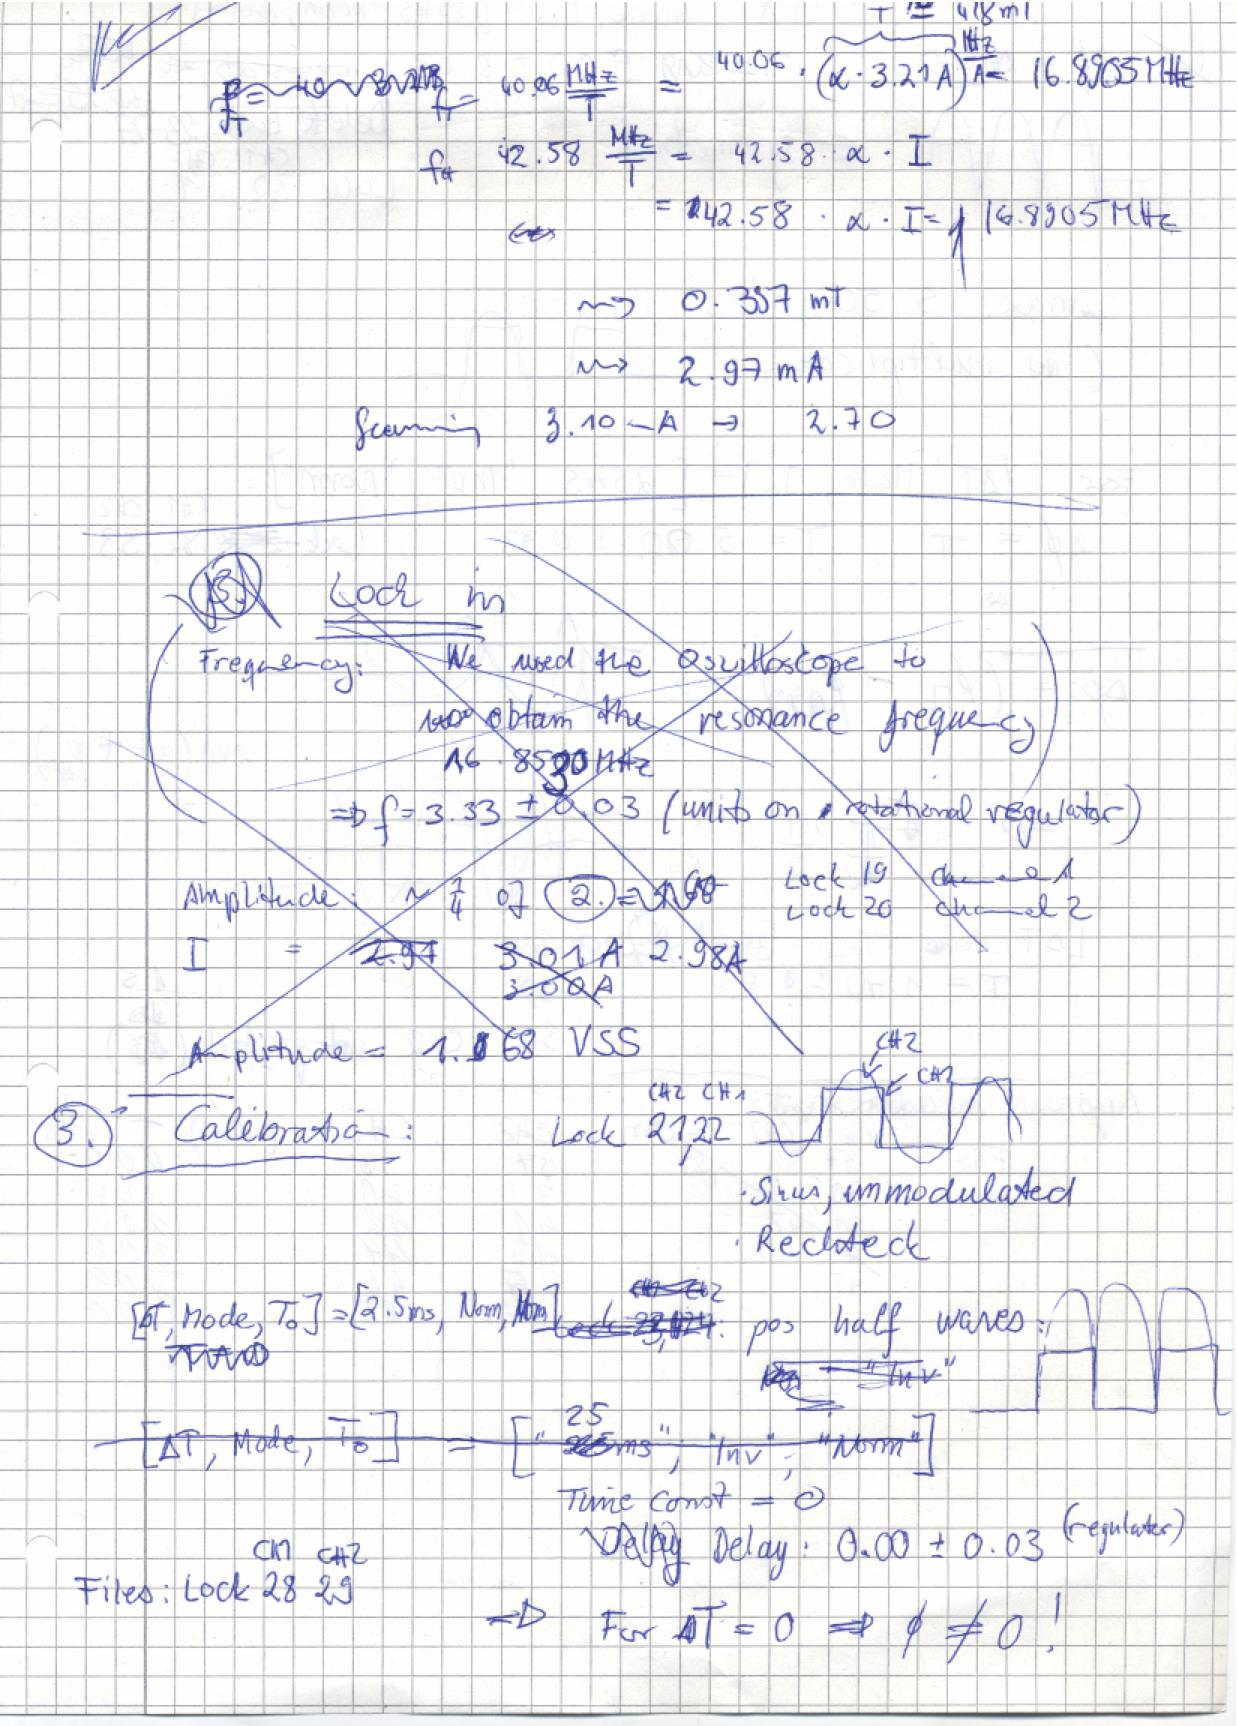
\includegraphics[width=\linewidth]{appendix/spin6.jpg}
\clearpage
    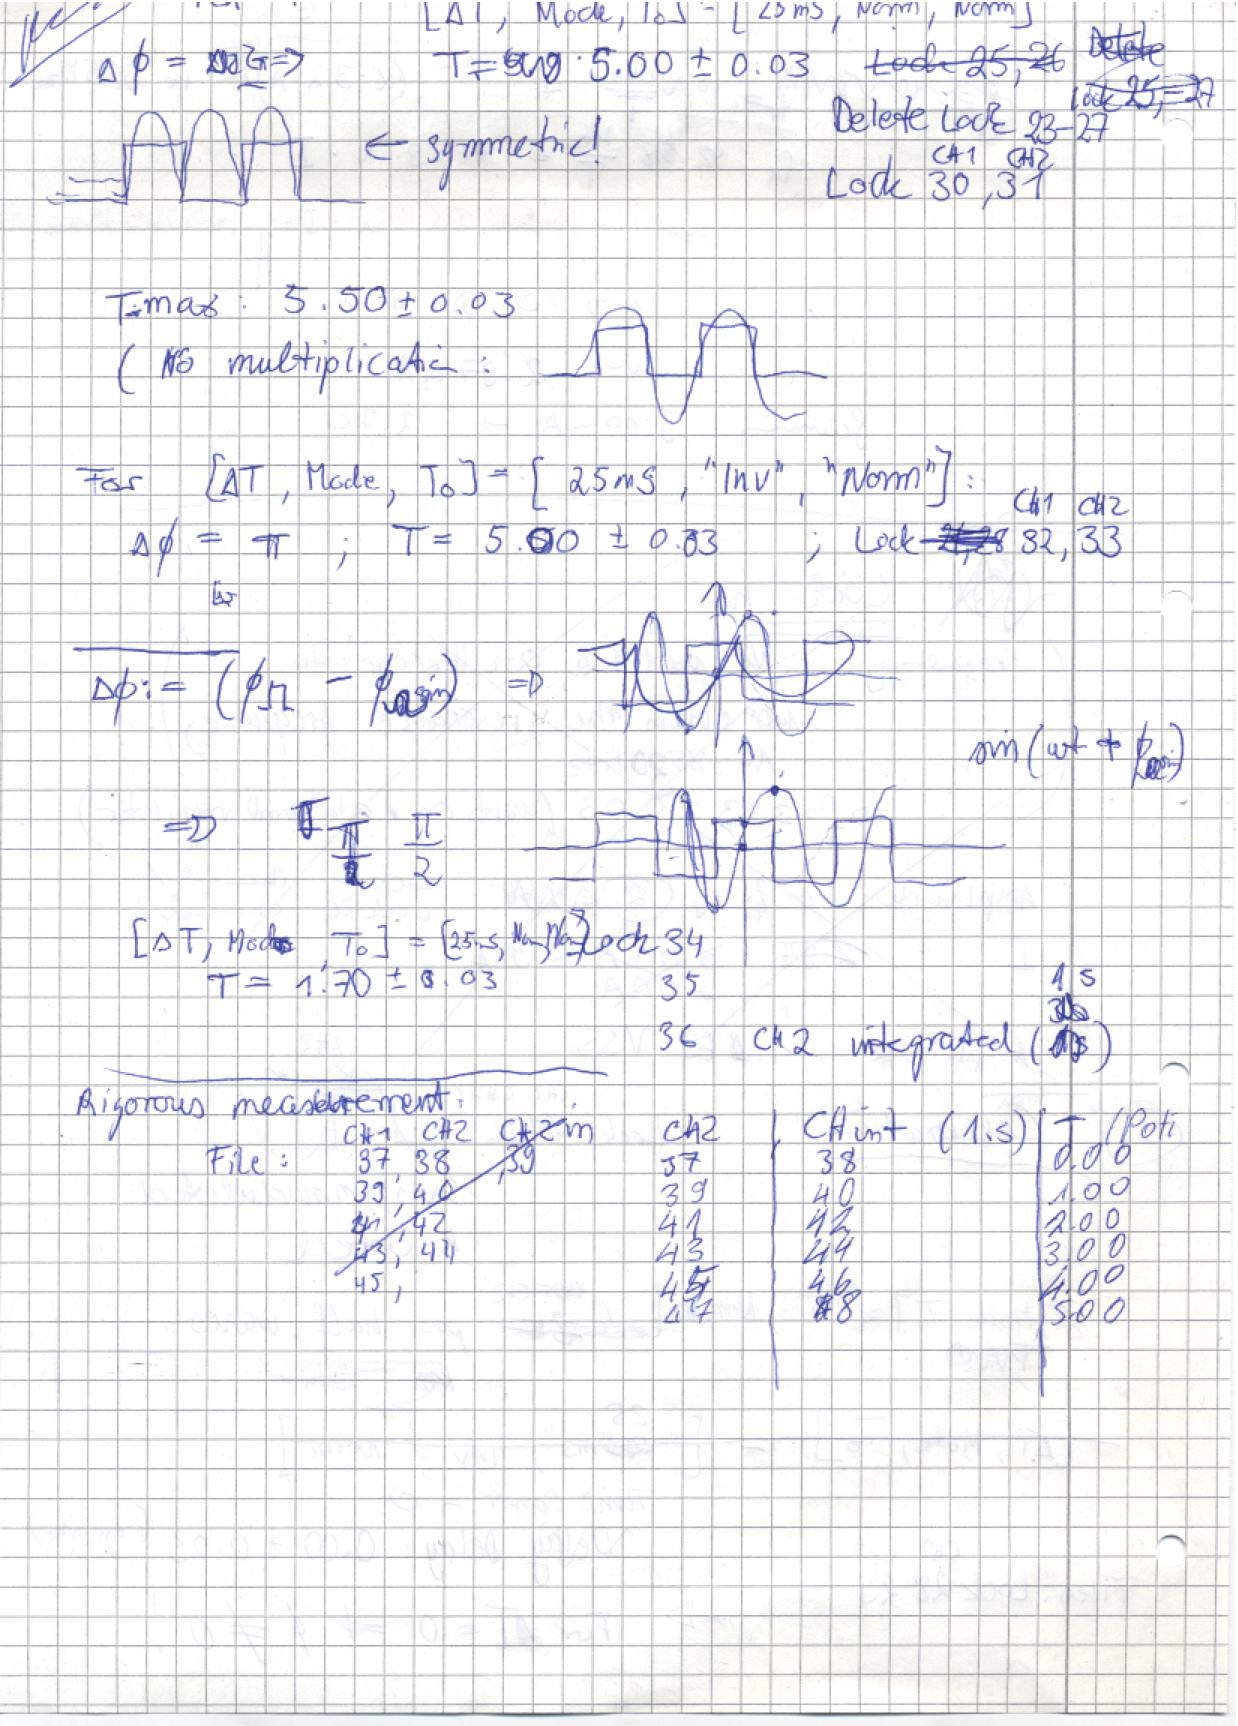
\includegraphics[width=\linewidth]{appendix/spin7.jpg}
\clearpage


\end{document}
